\documentclass[9pt]{beamer}
\mode<presentation>

% Theme choice:
\usetheme{Madrid}%Darmstadt 
\usepackage{xcolor}
\definecolor{mGreen}{rgb}{0,0.6,0}
\definecolor{mRed}{rgb}{0.6,0,0}
\usecolortheme[RGB={0,100,50}]{structure}
 \usefonttheme{structurebold} 
\setbeamercovered{invisible}
%\setbeamertemplate{navigation symbols}{}
\usepackage{dynblocks}
\usepackage{textpos}
\usepackage{amsfonts}
\usepackage{amsmath}
\usepackage{amssymb}
\usepackage{amsthm}
\usepackage{listings}
\usepackage{tikz}
\usepackage{pgfplots}
\pgfplotsset{compat=1.18}
\usetikzlibrary{
  arrows.meta,
  positioning,
  calc,
  fit,
  shapes.geometric,
  shapes.misc
}
\newtheorem{teorema}{Teorema}\usepackage{mathtools}
\renewcommand{\proofname}{Prova}
\usepackage[portuguese]{babel}

\uselanguage{Portuguese}
\languagepath{Portuguese}

\deftranslation[to=Portuguese]{Theorem}{Teorema}
\deftranslation[to=Portuguese]{Lemma}{Lema}
\deftranslation[to=Portuguese]{Corollary}{Corolário}
\deftranslation[to=Portuguese]{Proof}{Prova}

\usepackage{dutchcal}
\usepackage[utf8]{inputenc}
\usepackage[T1]{fontenc}
\usepackage{booktabs}
\usepackage[affil-it]{authblk} 
\usepackage{etoolbox}
\usepackage{lmodern}
\usepackage[pscoord]{eso-pic}
\usepackage{hyperref}

\makeatletter
\patchcmd{\@maketitle}{\LARGE \@title}{\fontsize{18}{19.2}\selectfont\@title}{}{}
\makeatother

\renewcommand\Authfont{\fontsize{12}{14.4}\selectfont}
\renewcommand\Affilfont{\fontsize{9}{10.8}\itshape}

% Estilos TikZ reutilizáveis (tema verde da apresentação)
\tikzset{
  softbox/.style={
    draw=structure.fg,
    fill=structure.fg!12,
    rounded corners=3pt,
    align=center,
    font=\small,
    minimum height=0.9cm,
    inner sep=4pt
  },
  softboxalert/.style={
    draw=mRed,
    fill=mRed!10,
    rounded corners=3pt,
    align=center,
    font=\small,
    minimum height=0.9cm,
    inner sep=4pt
  },
  softcore/.style={
    draw=structure.fg,
    fill=structure.fg!25,
    circle,
    align=center,
    font=\bfseries\small,
    minimum size=1.55cm,
    inner sep=2pt
  },
  softarrow/.style={
    -{Latex[length=2.2mm]},
    thick,
    structure.fg
  },
  softarrowalert/.style={
    -{Latex[length=2.2mm]},
    thick,
    mRed
  },
  softlabel/.style={font=\scriptsize\bfseries, text=structure.fg},
  % Mockups de interface gráfica
  guiwin/.style={
    draw=#1!70!black,
    fill=white,
    rounded corners=2pt,
    inner sep=0pt,
    thick
  },
  guibar/.style={
    draw=none,
    fill=#1,
    minimum height=0.32cm,
    inner sep=1pt,
    font=\tiny\bfseries,
    text=white,
    anchor=north west
  },
  guibtn/.style={
    circle,
    fill=#1,
    minimum size=0.14cm,
    inner sep=0pt
  },
  guiphone/.style={
    draw=#1!80!black,
    fill=black!85,
    rounded corners=6pt, 
    thick,
    inner sep=2pt
  }
}

% Title page details: 
\title[Presentation]{Introdução aos tópicos de base e terminologias essenciais segundo Engenharia de Software: Uma Abordagem Profissional} %add title

\institute[UniRV]{\large PROCESSO DE SOFTWARE --- Professor: Me. Sergio Souza Novak --- Faculdade de Engenharia de Software}
% \titlegraphic{\includegraphics[width=5cm]{msu.eps}}
\titlegraphic{
\includegraphics[width=5cm]{Universidade_de_Rio_Verde.jpg}}
\date{}
 
% Logo only on title page
%\logo{
\includegraphics[width=1cm,keepaspectratio]{Logo.png}}


\begin{document}

% Title page frame
\frame[plain]{\titlepage}
%logo
\AddToShipoutPictureFG{
    \put(\LenToUnit{.92\paperwidth},
    \LenToUnit{.185\paperheight})
    {\vtop{{\null}
    \makebox{
\includegraphics[width=.8cm,keepaspectratio]{Universidade_de_Rio_Verde.jpg}}}}}

\begin{frame}{Sumário}
  \tableofcontents
\end{frame}
\section{Disponibilidade de serviços e desafios}
% Slide 1: Introdução a Fermat
\section{1.1 A Natureza do Software}

%------------------------------------------------
\begin{frame}
\frametitle{1.1 A Natureza do Software}

\begin{block}{Conceito}
Software é o conjunto de programas, dados e documentação que
permite ao computador executar tarefas e resolver problemas.
\end{block}

\begin{columns}[T]
\column{0.48\textwidth}
\begin{itemize}
    \item Não é um componente físico.
    \item Controla o funcionamento do hardware.
    \item Processa, armazena e transmite informações.
\end{itemize}

\column{0.48\textwidth}
\begin{center}
\begin{tikzpicture}[node distance=0.35cm, scale=0.85]
  \node[softcore] (sw) {Software};
  \node[softbox, above=of sw, minimum width=2.1cm] (prog) {Programas};
  \node[softbox, left=0.4cm of sw, minimum width=1.45cm] (dados) {Dados};
  \node[softbox, right=0.4cm of sw, minimum width=1.9cm] (docs) {Docs};
  \node[softbox, below=of sw, minimum width=2.3cm] (hw) {Hardware};
  \draw[softarrow] (prog) -- (sw);
  \draw[softarrow] (dados) -- (sw);
  \draw[softarrow] (docs) -- (sw);
  \draw[softarrow] (sw) -- (hw);
\end{tikzpicture}
\end{center}
\end{columns}

\vspace{0.15cm}
\begin{alertblock}{Importância}
Vivemos na era da informação, e o software é o principal meio de
criação, processamento e distribuição dessa informação.
\end{alertblock}

\end{frame}

%------------------------------------------------
\begin{frame}
\frametitle{O Duplo Papel do Software}

\begin{center}
\begin{tikzpicture}[node distance=0.55cm]
  \node[softcore, minimum size=1.7cm] (centro) {Software};
  \node[softbox, left=1.35cm of centro, minimum width=3.2cm, text width=2.95cm] (produto) {%
    \textbf{Como Produto}\\[2pt]
    {\scriptsize Executa tarefas\\ Resolve problemas\\ Agrega valor ao HW}};
  \node[softbox, right=1.35cm of centro, minimum width=3.2cm, text width=2.95cm] (veiculo) {%
    \textbf{Como Veículo}\\[2pt]
    {\scriptsize Controla dispositivos\\ Comunicação\\ Cria outros softwares}};
  \draw[softarrow] (centro) -- (produto);
  \draw[softarrow] (centro) -- (veiculo);
\end{tikzpicture}
\end{center}

\vspace{0.25cm}

\begin{columns}
\column{0.48\textwidth}
\begin{block}{Exemplos --- Produto}
\begin{itemize}
    \item Microsoft Word, WhatsApp
    \item Photoshop, Sistema Bancário
\end{itemize}
\end{block}

\column{0.48\textwidth}
\begin{block}{Exemplos --- Veículo}
\begin{itemize}
    \item Windows, Linux, Android
    \item Compiladores
\end{itemize}
\end{block}
\end{columns}

\end{frame}

%------------------------------------------------
\begin{frame}
\frametitle{Software como Transformador de Informações}

\begin{center}
\begin{tikzpicture}[
  node distance=0.55cm and 0.35cm,
  box/.style={softbox, minimum width=2.35cm, minimum height=1.05cm, text width=2.15cm}
]
  \node[box] (dados) {Dados};
  \node[box, right=of dados] (proc) {Processamento};
  \node[box, right=of proc] (info) {Informação};
  \node[box, right=of info] (dec) {Conhecimento\\[-1pt]{\tiny para decisão}};
  \draw[softarrow] (dados) -- (proc);
  \draw[softarrow] (proc) -- (info);
  \draw[softarrow] (info) -- (dec);
  \node[softlabel, above=0.12cm of proc] {Software};
\end{tikzpicture}
\end{center}

\vspace{0.35cm}

O software pode:

\begin{columns}[T]
\column{0.48\textwidth}
\begin{itemize}
    \item Produzir informações;
    \item Armazenar dados;
    \item Modificar conteúdos;
\end{itemize}
\column{0.48\textwidth}
\begin{itemize}
    \item Exibir resultados;
    \item Compartilhar informações pela Internet.
\end{itemize}
\end{columns}

\end{frame}

%------------------------------------------------
\begin{frame}
\frametitle{Onde o Software Está Presente?}

\begin{center}
\begin{tikzpicture}[node distance=0.35cm]
  \node[softcore, minimum size=1.7cm] (c) {Software};
  \node[softbox, above left=0.55cm and 1.6cm of c, minimum width=2.5cm] (pc) {Computadores\\[-1pt]{\tiny Windows, Linux}};
  \node[softbox, above right=0.55cm and 1.6cm of c, minimum width=2.5cm] (mob) {Celulares\\[-1pt]{\tiny Android, iOS}};
  \node[softbox, left=1.7cm of c, minimum width=2.3cm] (cloud) {Nuvem\\[-1pt]{\tiny Drive, OneDrive}};
  \node[softbox, right=1.7cm of c, minimum width=2.5cm] (car) {Automóveis\\[-1pt]{\tiny Controle do motor}};
  \node[softbox, below left=0.55cm and 1.6cm of c, minimum width=2.5cm] (hosp) {Hospitais\\[-1pt]{\tiny Diagnóstico}};
  \node[softbox, below right=0.55cm and 1.6cm of c, minimum width=2.5cm] (agro) {Agricultura\\[-1pt]{\tiny Precisão}};
  \node[softbox, below=0.85cm of c, minimum width=3.2cm] (ind) {Indústria / Internet\\[-1pt]{\tiny Automação, e-commerce}};
  \foreach \n in {pc,mob,cloud,car,hosp,agro,ind}
    \draw[softarrow] (c) -- (\n);
\end{tikzpicture}
\end{center}

\end{frame}

%------------------------------------------------
\begin{frame}
\frametitle{O Software Distribui Informação}

O principal produto distribuído pelo software é a informação.

\vspace{0.15cm}

\begin{center}
\begin{tikzpicture}[
  node distance=0.4cm and 0.3cm,
  stepbox/.style={softbox, minimum width=2.1cm, minimum height=0.95cm, text width=1.95cm, font=\scriptsize}
]
  \node[stepbox] (a) {Autenticação};
  \node[stepbox, right=of a] (b) {Pagamento};
  \node[stepbox, right=of b] (c) {Estoque};
  \node[stepbox, right=of c] (d) {Nota fiscal};
  \draw[softarrow] (a) -- (b);
  \draw[softarrow] (b) -- (c);
  \draw[softarrow] (c) -- (d);
  \node[softlabel, above=0.05cm of b] {Compra online --- fluxo};
\end{tikzpicture}
\end{center}

\vspace{0.2cm}

\begin{columns}[T]
\column{0.48\textwidth}
\begin{itemize}
\item Dados financeiros e comerciais
\item Sistemas governamentais
\item Comunicação pela Internet
\end{itemize}
\column{0.48\textwidth}
\begin{itemize}
\item Redes sociais
\item Inteligência Artificial
\item Serviços em nuvem
\end{itemize}
\end{columns}

\end{frame}

%------------------------------------------------
\begin{frame}
\frametitle{Benefícios e Desafios do Software}

\begin{center}
\begin{tikzpicture}[node distance=0.55cm]
  \node[softbox, minimum width=4.4cm, text width=4.1cm, align=left] (ben) {%
    \textbf{Benefícios}\\[3pt]
    {\scriptsize
    Automação $\cdot$ Rapidez $\cdot$ Precisão\\
    Comunicação global\\
    Compartilhamento $\cdot$ IA}};
  \node[softboxalert, right=1.3cm of ben, minimum width=4.4cm, text width=4.1cm, align=left] (des) {%
    \textbf{Desafios}\\[3pt]
    {\scriptsize
    Ataques cibernéticos\\
    Vazamento de dados $\cdot$ Fraudes\\
    Privacidade $\cdot$ Dependência}};
  \node[softcore, minimum size=1.35cm] at ($(ben)!0.5!(des)$) {SW};
  \draw[softarrow] (ben.east) -- ++(0.15,0);
  \draw[softarrowalert] (des.west) -- ++(-0.15,0);
\end{tikzpicture}
\end{center}

\vspace{0.35cm}

\begin{alertblock}{Equilíbrio}
O mesmo poder que gera benefícios amplia a superfície de risco:
segurança e ética tornam-se requisitos de projeto.
\end{alertblock}

\end{frame}

%------------------------------------------------
\begin{frame}
\frametitle{Evolução do Software}

\begin{center}
\begin{tikzpicture}[
  node distance=0.15cm,
  era/.style={softbox, minimum width=3.1cm, minimum height=2.35cm, text width=2.9cm, font=\scriptsize, align=center}
]
  \node[era] (e1) {%
    \textbf{Décadas iniciais}\\[4pt]
    Programador\\trabalhando\\sozinho};
  \node[era, right=0.45cm of e1] (e2) {%
    \textbf{1980--2000}\\[4pt]
    Equipes pequenas\\e sistemas\\corporativos};
  \node[era, right=0.45cm of e2] (e3) {%
    \textbf{Atualmente}\\[4pt]
    Grandes equipes,\\nuvem, IA,\\microserviços, IoT};
  \draw[softarrow] (e1) -- (e2);
  \draw[softarrow] (e2) -- (e3);
  \node[softlabel, below=0.2cm of e2] {Complexidade crescente $\longrightarrow$};
\end{tikzpicture}
\end{center}

\vspace{0.45cm}

A evolução do hardware permitiu o desenvolvimento de softwares
cada vez mais complexos.

\end{frame}

%------------------------------------------------
\begin{frame}
\frametitle{O Crescimento da Complexidade}

\begin{columns}[T]
\column{0.48\textwidth}
Os sistemas atuais possuem:

\begin{itemize}
\item Milhões de linhas de código;
\item Milhares de usuários simultâneos;
\item Comunicação entre dezenas de serviços;
\item Armazenamento em nuvem;
\item Inteligência Artificial integrada;
\item Alta disponibilidade e segurança.
\end{itemize}

\column{0.48\textwidth}
\begin{center}
\begin{tikzpicture}[
  layer/.style={softbox, minimum width=4.2cm, minimum height=0.72cm, font=\scriptsize}
]
  \node[layer] (l1) {Usuários};
  \node[layer, below=0.28cm of l1] (l2) {Aplicações / IA};
  \node[layer, below=0.28cm of l2] (l3) {Microserviços};
  \node[layer, below=0.28cm of l3] (l4) {Nuvem / Dados};
  \node[layer, below=0.28cm of l4] (l5) {Infraestrutura};
  \draw[softarrow] (l1) -- (l2);
  \draw[softarrow] (l2) -- (l3);
  \draw[softarrow] (l3) -- (l4);
  \draw[softarrow] (l4) -- (l5);
\end{tikzpicture}
\end{center}
\end{columns}

\vspace{0.25cm}
\begin{alertblock}{Consequência}
Quanto maior a complexidade, maior a necessidade de planejamento,
projeto, testes e manutenção.
\end{alertblock}

\end{frame}

%------------------------------------------------
\begin{frame}
\frametitle{Os Grandes Desafios do Desenvolvimento}

Mesmo com tecnologias modernas, várias perguntas continuam atuais:

\vspace{0.2cm}

\begin{center}
\begin{tikzpicture}[
  node distance=0.35cm and 0.4cm,
  q/.style={softboxalert, minimum width=4.6cm, text width=4.3cm, font=\scriptsize, align=left}
]
  \node[q] (q1) {1. Por que demora tanto para ficar pronto?};
  \node[q, right=of q1] (q2) {2. Por que o desenvolvimento custa caro?};
  \node[q, below=of q1] (q3) {3. Por que ainda existem tantos erros?};
  \node[q, right=of q3] (q4) {4. Por que a manutenção consome tanto tempo?};
  \node[q, below=0.35cm of $(q3)!0.5!(q4)$, minimum width=9.6cm, text width=9.3cm] (q5)
    {5. Como medir corretamente o progresso do projeto?};
\end{tikzpicture}
\end{center}

\end{frame}

%------------------------------------------------
\begin{frame}
\frametitle{A Engenharia de Software}

\begin{center}
\begin{tikzpicture}[node distance=0.45cm]
  \node[softcore, minimum size=1.9cm, text width=1.5cm] (es) {Engenharia\\de\\Software};
  \node[softbox, above left=0.5cm and 1.5cm of es, minimum width=2.4cm] (proc) {Processos};
  \node[softbox, above right=0.5cm and 1.5cm of es, minimum width=2.4cm] (met) {Métodos};
  \node[softbox, below left=0.5cm and 1.5cm of es, minimum width=2.4cm] (ferr) {Ferramentas};
  \node[softbox, below right=0.5cm and 1.5cm of es, minimum width=2.4cm] (prat) {Boas práticas};
  \foreach \n in {proc,met,ferr,prat}
    \draw[softarrow] (\n) -- (es);
\end{tikzpicture}
\end{center}

\vspace{0.2cm}

\begin{block}{Objetivo}
Produzir software com qualidade, menor custo e tempo,
maior confiabilidade e facilidade de manutenção.
\end{block}

\end{frame}

%------------------------------------------------
\begin{frame}
\frametitle{Resumo}

\begin{columns}[T]
\column{0.55\textwidth}
\begin{itemize}
\item Software é produto e veículo.
\item Transforma dados em decisão.
\item Está em todas as áreas.
\item Complexidade crescente.
\item Desafios de prazo, custo e qualidade.
\item A ES organiza o desenvolvimento.
\end{itemize}

\column{0.43\textwidth}
\begin{center}
\begin{tikzpicture}[node distance=0.32cm]
  \node[softbox, minimum width=3.6cm] (a) {Natureza};
  \node[softbox, below=of a, minimum width=3.6cm] (b) {Papéis};
  \node[softbox, below=of b, minimum width=3.6cm] (c) {Complexidade};
  \node[softbox, below=of c, minimum width=3.6cm] (d) {Eng. de Software};
  \draw[softarrow] (a) -- (b);
  \draw[softarrow] (b) -- (c);
  \draw[softarrow] (c) -- (d);
\end{tikzpicture}
\end{center}
\end{columns}

\vfill

\centering
\Large
``Software é o elemento que dá inteligência ao hardware.''

\end{frame}



%------------------------------------------------
\begin{frame}
\frametitle{Definição de Software}

\begin{columns}

\column{0.40\textwidth}

\begin{block}{Definição}
Software é composto por:
\begin{itemize}
    \item Programas;
    \item Estruturas de dados;
    \item Documentação.
\end{itemize}
\end{block}

\column{0.60\textwidth}

\centering
\begin{tikzpicture}[
scale=0.3,
caixa/.style={
draw,
rounded corners,
thick,
minimum width=1.8cm,
minimum height=0.9cm,
align=center,
fill=blue!10
},
seta/.style={-Latex,thick}
]

\node[caixa] (prog) {Programas};

\node[caixa,below=8mm of prog] (dados)
{Estruturas\\de Dados};

\node[caixa,below=8mm of dados] (doc)
{Documentação};

\node[caixa,right=3cm of dados,fill=green!15] (soft)
{\Large Software};

\draw[seta] (prog.east)--(soft.west);
\draw[seta] (dados.east)--(soft.west);
\draw[seta] (doc.east)--(soft.west);

\end{tikzpicture}

\end{columns}

\vspace{0.4cm}

\begin{alertblock}{Importante}
Software não é apenas código. Dados e documentação também fazem
parte do produto.
\end{alertblock}

\end{frame}
%------------------------------------------------
\begin{frame}
    \frametitle{Os Componentes do Software}
    
    \centering
    
    \begin{tikzpicture}[
    caixa/.style={
    draw,
    rounded corners,
    minimum width=3cm,
    minimum height=1cm,
    align=center,
    fill=cyan!15,
    thick
    },
    seta/.style={-Latex,thick}
    ]
    
    \node[caixa] (soft) at (0,3)
    {\Large Software};
    
    \node[caixa] (prog) at (-4,0)
    {\textbf{Programas}\\Instruções};
    
    \node[caixa] (dados) at (0,0)
    {\textbf{Dados}\\Informações};
    
    \node[caixa] (doc) at (4,0)
    {\textbf{Documentação}\\Manuais};
    
    \draw[seta] (soft)--(prog);
    \draw[seta] (soft)--(dados);
    \draw[seta] (soft)--(doc);
    
    \end{tikzpicture}
    
    \vspace{0.6cm}
    
    \begin{block}{Exemplo}
    Um sistema bancário possui código-fonte, banco de dados dos clientes,
    documentação técnica e manual do usuário.
    \end{block}
    
    \end{frame}
    %------------------------------------------------


    %=========================================================
% Curvas de Defeitos - Hardware e Software
%=========================================================

%---------------------------------------------------------
\begin{frame}
    \frametitle{A Curva da Banheira (Hardware)}
    
    \begin{columns}
    
    \column{0.55\textwidth}
    
    \begin{itemize}
    \item O hardware é um componente físico.
    
    \item Sua taxa de defeitos varia durante sua vida útil.
    
    \item Esse comportamento é conhecido como
    \textbf{Curva da Banheira}.
    
    \item A curva apresenta três fases bem definidas.
    \end{itemize}
    
    \column{0.45\textwidth}
    
    \centering
    
    \begin{tikzpicture}[
    scale=0.72,
    >=Latex
    ]
    
    \draw[->,thick] (0,0)--(6.5,0)
    node[right]{Tempo};
    
    \draw[->,thick] (0,0)--(0,4.5)
    node[above,rotate=90]{Taxa de defeitos};
    
    \draw[very thick]
    plot[smooth]
    coordinates{
    (0.5,4)
    (1.0,2.3)
    (2.0,0.8)
    (3.6,0.55)
    (5.1,0.75)
    (5.8,1.6)
    (6.2,4)
    };
    
    \end{tikzpicture}
    
    \end{columns}
    
    \end{frame}
    
    %---------------------------------------------------------
    \begin{frame}
    \frametitle{As Três Fases da Vida do Hardware}
    
    \centering
    
    \begin{tikzpicture}[
    scale=0.95,
    >=Latex
    ]
    
    % Eixos
    \draw[->,thick] (0,0)--(10.5,0)
    node[right]{Tempo};
    
    \draw[->,thick] (0,0)--(0,5)
    node[above,rotate=90]{Taxa de defeitos};
    
    % Curva
    \draw[very thick]
    plot[smooth]
    coordinates{
    (0.7,4.4)
    (1.6,2.2)
    (3.0,0.8)
    (7.2,0.8)
    (8.5,1.0)
    (9.2,2.2)
    (10.0,4.5)
    };
    
    % divisões
    \draw[dashed] (3,0)--(3,5);
    \draw[dashed] (8.3,0)--(8.3,5);
    
    % rótulos
    \node[align=center] at (1.4,4.2)
    {\small Mortalidade\\Infantil};
    
    \node at (5.6,4.2)
    {\small Vida útil};
    
    \node at (9.2,4.2)
    {\small Desgaste};
    
    \end{tikzpicture}
    
    \vspace{0.4cm}
    
    \begin{block}{Interpretação}
    
    \begin{enumerate}
    \item Alta taxa inicial devido a defeitos de fabricação ou projeto.
    \item Longo período com poucas falhas.
    \item Aumento das falhas devido ao desgaste físico dos componentes.
    \end{enumerate}
    
    \end{block}
    
    \end{frame}
    
    %---------------------------------------------------------
    \begin{frame}
    \frametitle{Hardware x Software}
    
    \begin{columns}
    
    \column{0.48\textwidth}
    
    \begin{block}{Hardware}
    
    \begin{itemize}
    \item Componente físico.
    \item Sofre desgaste.
    \item Poeira.
    \item Vibração.
    \item Calor.
    \item Corrosão.
    \item Necessita substituição de peças.
    \end{itemize}
    
    \end{block}
    
    \column{0.48\textwidth}
    
    \begin{block}{Software}
    
    \begin{itemize}
    \item Produto lógico.
    \item Não sofre desgaste físico.
    \item Não envelhece.
    \item Defeitos são erros de projeto.
    \item Não existem peças de reposição.
    \end{itemize}
    
    \end{block}
    
    \end{columns}
    
    \vspace{0.4cm}
    
    \begin{alertblock}{Conclusão}
    
    Enquanto o hardware envelhece fisicamente, o software somente muda
    quando é corrigido ou modificado.
    
    \end{alertblock}
    
    \end{frame}
    
    %---------------------------------------------------------
    \begin{frame}
    \frametitle{Curva Idealizada de Defeitos do Software}
    
    \begin{columns}
    
    \column{0.55\textwidth}
    
    \begin{itemize}
    
    \item Muitos defeitos são encontrados logo após o desenvolvimento.
    
    \item As correções reduzem rapidamente a taxa de falhas.
    
    \item Após as correções, espera-se uma taxa praticamente constante.
    
    \item Diferentemente do hardware, não existe desgaste físico.
    
    \end{itemize}
    
    \column{0.45\textwidth}
    
    \centering
    
    \begin{tikzpicture}[
    scale=0.72,
    >=Latex
    ]
    
    \draw[->,thick] (0,0)--(6.5,0)
    node[right]{Tempo};
    
    \draw[->,thick] (0,0)--(0,4.5)
    node[above,rotate=90]{Taxa de defeitos};
    
    \draw[very thick]
    plot[smooth]
    coordinates{
    (0.5,4)
    (1.1,2.1)
    (1.8,1.0)
    (2.7,0.45)
    (6.0,0.45)
    };
    
    \node at (4.9,0.9)
    {\small Curva idealizada};
    
    \end{tikzpicture}
    
    \end{columns}
    
    \end{frame}
    
    %---------------------------------------------------------
    \begin{frame}
    \frametitle{Curva Real de Defeitos do Software}
    
    \centering
    
    \begin{tikzpicture}[
    scale=0.82,
    >=Latex
    ]
    
    % eixos
    \draw[->,thick] (0,0)--(11,0)
    node[right]{Tempo};
    
    \draw[->,thick] (0,0)--(0,5)
    node[above,rotate=90]{Taxa de defeitos};
    
    % curva ideal
    \draw[very thick]
    plot[smooth]
    coordinates{
    (0.8,4.2)
    (1.7,2.1)
    (2.8,0.7)
    (10,0.7)
    };
    
    \node[right] at (10.1,0.7)
    {\small Idealizada};
    
    % curva real
    \draw[thick]
    plot[smooth]
    coordinates{
    (0.8,4.2)
    (1.7,2.1)
    (2.8,1.1)
    };
    
    \fill (2.8,1.1) circle (2.5pt);
    
    \node[below] at (2.8,1.0)
    {\scriptsize Mudança};
    
    \draw[thick] (2.8,1.1)--(2.8,3.7);
    
    \draw[thick]
    plot[smooth]
    coordinates{
    (2.8,3.7)
    (3.8,2.2)
    (4.8,1.5)
    };
    
    \draw[thick] (4.8,1.5)--(4.8,3.6);
    
    \draw[thick]
    plot[smooth]
    coordinates{
    (4.8,3.6)
    (5.8,2.3)
    (6.8,1.8)
    };
    
    \draw[thick] (6.8,1.8)--(6.8,3.8);
    
    \draw[thick]
    plot[smooth]
    coordinates{
    (6.8,3.8)
    (7.8,2.6)
    (9.8,2.2)
    };
    
    \node[right] at (9.9,2.2)
    {\small Curva real};
    
    % seta
    \draw[->] (7.2,4.4)--(6.9,3.9);
    
    \node[align=center] at (6.4,4.7)
    {\small Aumento da taxa\\de defeitos devido\\às modificações};
    
    \end{tikzpicture}
    
    \vspace{0.35cm}
    
    \begin{alertblock}{Conclusão}
    
    Cada manutenção ou nova funcionalidade pode introduzir novos
    erros. Assim, o software \textbf{não se desgasta}, mas pode
    \textbf{deteriorar devido às modificações realizadas ao longo de sua vida}.
    
    \end{alertblock}
    
    \end{frame}
    
    %---------------------------------------------------------
    \begin{frame}
    \frametitle{Resumo}
    
    \begin{center}
    
    \begin{tikzpicture}[
    caixa/.style={
    draw,
    rounded corners,
    minimum width=4.2cm,
    minimum height=1cm,
    align=center,
    fill=blue!10,
    thick
    },
    seta/.style={-Latex,thick}
    ]
    
    \node[caixa] (hw)
    {Hardware};
    
    \node[caixa,right=4cm of hw]
    (sw){Software};
    
    \node[caixa,below=1.8cm of hw]
    (hw2){Desgasta-se\\fisicamente};
    
    \node[caixa,below=1.8cm of sw]
    (sw2){Deteriora\\pelas modificações};
    
    \draw[seta](hw)--(hw2);
    \draw[seta](sw)--(sw2);
    
    \end{tikzpicture}
    
    \end{center}
    
    \vspace{0.5cm}
    
    \begin{block}{Mensagem Principal}
    
    \begin{itemize}
    
    \item Hardware falha devido ao envelhecimento dos componentes.
    
    \item Software não sofre desgaste físico.
    
    \item A manutenção e a evolução do software podem introduzir novos defeitos.
    
    \item Quanto maior o número de modificações, maior a necessidade de testes e controle de qualidade.
    
    \end{itemize}
    
    \end{block}
    
    \end{frame}


    %%%%%%%%%%%%%%%%%%%%%%%%%%%%%%%%%%%%%%%%%%%%%%%%%%%%%%%%%%%%%%
%% 1.1.2 Domínios de Aplicação de Software
%%%%%%%%%%%%%%%%%%%%%%%%%%%%%%%%%%%%%%%%%%%%%%%%%%%%%%%%%%%%%%

%-------------------------------------------------------------
\begin{frame}
\frametitle{1.1.2 Domínios de Aplicação de Software}

{\small Como classificar? Observe \textbf{onde} o software roda e \textbf{para quem} ele trabalha.}

\vspace{0.15cm}
\begin{center}
\begin{tikzpicture}[scale=0.9,
  h/.style={font=\scriptsize\bfseries, align=center},
  c/.style={font=\tiny, align=center, text width=2.15cm},
  box/.style={draw=structure.fg!50, rounded corners=2pt, minimum height=0.72cm, text width=2.15cm, align=center, font=\tiny, inner sep=2pt}
]
\node[h] at (0,3.2) {Domínio};
\node[h] at (2.6,3.2) {Onde roda?};
\node[h] at (5.2,3.2) {Para quem?};
\node[h] at (7.8,3.2) {Exemplo famoso};

\draw[structure.fg!40, thick] (-1.2,2.9) -- (9.0,2.9);

\node[box, fill=blue!12] at (0,2.35) {Sistema};
\node[c] at (2.6,2.35) {PC / celular\\(camada base)};
\node[c] at (5.2,2.35) {Outros programas};
\node[c] at (7.8,2.35) {Windows, Android};

\node[box, fill=orange!15] at (0,1.55) {Aplicação};
\node[c] at (2.6,1.55) {Desktop / nuvem};
\node[c] at (5.2,1.55) {Usuário final};
\node[c] at (7.8,1.55) {Word, Photoshop};

\node[box, fill=cyan!15] at (0,0.75) {Científico};
\node[c] at (2.6,0.75) {Workstation / HPC};
\node[c] at (5.2,0.75) {Pesquisador};
\node[c] at (7.8,0.75) {MATLAB, Jupyter};

\node[box, fill=yellow!20] at (0,-0.05) {Embarcado};
\node[c] at (2.6,-0.05) {Dentro do aparelho};
\node[c] at (5.2,-0.05) {Dispositivo};
\node[c] at (7.8,-0.05) {Carro, micro-ondas};

\node[box, fill=purple!12] at (0,-0.85) {Web/Mobile};
\node[c] at (2.6,-0.85) {Navegador / app};
\node[c] at (5.2,-0.85) {Milhões de usuários};
\node[c] at (7.8,-0.85) {Gmail, WhatsApp};

\node[box, fill=red!12] at (0,-1.65) {IA};
\node[c] at (2.6,-1.65) {Nuvem + modelo};
\node[c] at (5.2,-1.65) {Humanos + sistemas};
\node[c] at (7.8,-1.65) {ChatGPT, Netflix};
\end{tikzpicture}
\end{center}
\end{frame}

%-------------------------------------------------------------
\begin{frame}
\frametitle{1. Software de Sistema --- a ``fundação''}

\begin{alertblock}{Ideia-chave}
Sem o SO, Word/Chrome \textbf{não sobem}. O sistema operacional fica \emph{entre} o hardware e as aplicações.
\end{alertblock}

\begin{center}
\begin{tikzpicture}[scale=0.85]
  % Stack didática
  \fill[orange!25, rounded corners=3pt] (0,3.0) rectangle (5.8,3.9);
  \node[font=\small\bfseries] at (2.9,3.55) {Aplicações (Word, Chrome, jogos)};
  \node[font=\tiny, orange!70!black] at (7.3,3.45) {usam o SO};

  \fill[blue!25, rounded corners=3pt] (0,1.7) rectangle (5.8,2.85);
  \node[font=\small\bfseries] at (2.9,2.45) {Sistema Operacional};
  \node[font=\tiny] at (2.9,2.05) {Windows $\cdot$ Linux $\cdot$ Android};
  \node[font=\tiny, blue!70!black, text width=2.4cm, align=left] at (7.5,2.3)
    {gerencia CPU,\\memória, disco,\\rede e drivers};

  \fill[gray!35, rounded corners=3pt] (0,0.4) rectangle (5.8,1.55);
  \node[font=\small\bfseries] at (2.9,1.15) {Hardware};
  \node[font=\tiny] at (2.9,0.75) {CPU $\cdot$ RAM $\cdot$ disco $\cdot$ tela};

  \draw[softarrow] (2.9,3.0) -- (2.9,2.85);
  \draw[softarrow] (2.9,1.7) -- (2.9,1.55);

  % Mini Windows na lateral inferior como exemplo visual
  \begin{scope}[shift={(0,-1.55)}, scale=0.55]
    \draw[thick, fill=cyan!20] (0,0) rectangle (5.2,2.2);
    \fill[blue!75!black] (0,0) rectangle (5.2,0.35);
    \node[font=\tiny\bfseries,white] at (0.55,0.17) {Iniciar};
    \draw[fill=white] (1.4,0.55) rectangle (4.8,2.05);
    \fill[blue!70] (1.4,1.75) rectangle (4.8,2.05);
    \node[font=\tiny\bfseries,white] at (3.1,1.9) {Explorador};
    \node[font=\tiny\bfseries,blue!70!black] at (2.6,-0.35) {Ex.: interface do Windows};
  \end{scope}
\end{tikzpicture}
\end{center}
\end{frame}

%-------------------------------------------------------------
\begin{frame}
\frametitle{2. Software de Aplicação --- resolve um problema}

\begin{columns}[T]
\column{0.42\textwidth}
\begin{block}{Pergunta didática}
Qual \textbf{necessidade} do usuário este programa atende?
\end{block}
\begin{enumerate}
\item \textbf{Word} $\rightarrow$ escrever documentos
\item \textbf{Photoshop} $\rightarrow$ editar imagens
\item \textbf{App do banco} $\rightarrow$ pagar contas
\end{enumerate}
\vspace{0.1cm}
{\scriptsize Também: ERP, SIGAA, planilhas.}

\column{0.56\textwidth}
\centering
\begin{tikzpicture}[scale=0.78]
  % Fluxo problema -> app -> resultado
  \node[draw=mRed, fill=mRed!10, rounded corners, text width=2.4cm, align=center, font=\scriptsize]
    (prob) at (0,3.2) {Problema:\\``preciso do relatório''};
  \node[draw=blue!70, fill=blue!12, rounded corners, text width=2.6cm, align=center, font=\scriptsize\bfseries]
    (app) at (0,1.7) {Microsoft Word};
  \node[draw=structure.fg, fill=structure.fg!15, rounded corners, text width=2.4cm, align=center, font=\scriptsize]
    (ok) at (0,0.2) {Resultado:\\documento pronto};

  \draw[softarrowalert] (prob) -- node[right,font=\tiny]{escolhe a ferramenta} (app);
  \draw[softarrow] (app) -- node[right,font=\tiny]{usuário edita} (ok);

  % Mini Word anotado
  \begin{scope}[shift={(3.2,0.3)}]
    \draw[thick, fill=white] (0,0) rectangle (3.6,3.4);
    \fill[blue!65] (0,3.05) rectangle (3.6,3.4);
    \node[font=\tiny\bfseries,white] at (1.8,3.225) {Word};
    \fill[blue!8] (0,2.6) rectangle (3.6,3.05);
    \node[font=\tiny] at (0.7,2.82) {Arquivo};
    \node[font=\tiny] at (1.8,2.82) {Inserir};
    \fill[gray!12] (0.2,0.25) rectangle (3.4,2.45);
    \node[font=\tiny\bfseries,anchor=west] at (0.35,2.15) {Relatório};
    \foreach \y in {0,...,3}
      \draw[gray!45] (0.35,1.8-0.3*\y) -- (3.2,1.8-0.3*\y);
    % callout
    \draw[orange!80!black, thick] (0.3,2.5) rectangle (3.3,3.0);
    \node[font=\tiny,orange!80!black] at (1.8,3.65) {menus = ações do usuário};
  \end{scope}
\end{tikzpicture}
\end{columns}
\end{frame}

%-------------------------------------------------------------
\begin{frame}
\frametitle{3. Software Científico --- do dado ao gráfico}

\begin{block}{Ideia-chave}
Aqui o software é um \textbf{laboratório digital}: código $\rightarrow$ cálculo $\rightarrow$ visualização.
\end{block}

\begin{center}
\begin{tikzpicture}[scale=0.82]
  % Pipeline
  \node[draw, rounded corners, fill=cyan!15, minimum width=2.3cm, font=\scriptsize\bfseries] (d) at (0,2.2) {1. Dados};
  \node[draw, rounded corners, fill=orange!20, minimum width=2.3cm, font=\scriptsize\bfseries] (m) at (3.2,2.2) {2. Modelo};
  \node[draw, rounded corners, fill=blue!15, minimum width=2.3cm, font=\scriptsize\bfseries] (g) at (6.4,2.2) {3. Gráfico};
  \draw[softarrow] (d)--(m);
  \draw[softarrow] (m)--(g);
  \node[font=\tiny] at (1.6,2.65) {entrada};
  \node[font=\tiny] at (4.8,2.65) {simulação};
  \node[font=\tiny] at (6.4,1.7) {interpretação};

  % MATLAB canvas único com anotações
  \draw[thick, fill=white] (0.2,-0.9) rectangle (9.0,1.4);
  \fill[orange!70!black] (0.2,1.05) rectangle (9.0,1.4);
  \node[font=\tiny\bfseries,white,anchor=west] at (0.35,1.225) {MATLAB / Octave --- Figure 1};

  \fill[gray!10] (0.35,-0.7) rectangle (3.3,0.95);
  \node[font=\tiny\ttfamily,anchor=north west] at (0.45,0.9) {>> x = 0:0.1:10};
  \node[font=\tiny\ttfamily,anchor=north west] at (0.45,0.55) {>> y = sin(x)};
  \node[font=\tiny\ttfamily,anchor=north west] at (0.45,0.2) {>> plot(x,y)};
  \node[font=\tiny\bfseries,orange!70!black] at (1.8,-0.55) {comandos};

  \draw[thick,->] (3.7,-0.55)--(8.5,-0.55);
  \draw[thick,->] (3.7,-0.55)--(3.7,0.9);
  \draw[very thick,blue!70]
    plot[smooth] coordinates{(3.9,0.1)(4.5,0.7)(5.2,-0.1)(5.9,0.75)(6.6,0.0)(7.3,0.65)(8.2,0.15)};
  \node[font=\tiny] at (6.2,1.0) {resultado da simulação};

  \node[font=\tiny, text width=3.5cm, align=center] at (4.6,-1.25)
    {Exemplos: Jupyter, AutoCAD, ANSYS --- mesma lógica: calcular e visualizar};
\end{tikzpicture}
\end{center}
\end{frame}

%-------------------------------------------------------------
\begin{frame}
\frametitle{4. Software Embarcado --- software ``dentro'' do aparelho}

\begin{columns}[T]
\column{0.40\textwidth}
\begin{alertblock}{Diferença}
Você \textbf{não instala} um app: o programa já veio soldado/gravado no dispositivo.
\end{alertblock}
\begin{enumerate}
\item Sensor lê o mundo
\item Firmware decide
\item Atuador age
\end{enumerate}
{\scriptsize Exemplos: carro, micro-ondas, drone, equipamento médico.}

\column{0.60\textwidth}
\centering
\begin{tikzpicture}[scale=0.75]
  % Ciclo sensor-firmware-atuador
  \node[circle, draw=cyan!70!black, fill=cyan!20, minimum size=1.5cm, font=\scriptsize\bfseries, align=center] (s) at (0,2.2) {Sensor};
  \node[circle, draw=structure.fg, fill=structure.fg!25, minimum size=1.7cm, font=\scriptsize\bfseries, align=center] (f) at (2.4,0.6) {Firmware\\(SW)};
  \node[circle, draw=orange!80!black, fill=orange!25, minimum size=1.5cm, font=\scriptsize\bfseries, align=center] (a) at (0,-1.0) {Atuador};
  \draw[softarrow] (s) -- node[right,font=\tiny]{dado} (f);
  \draw[softarrow] (f) -- node[right,font=\tiny]{comando} (a);
  \draw[dashed, softarrow] (a.west) to[bend left=40] node[left,font=\tiny]{efeito} (s.west);

  % Mini painel carro como UI embutida
  \begin{scope}[shift={(4.0,0.2)}, scale=0.55]
    \fill[black!85, rounded corners=3pt] (0,0) rectangle (4.2,3.2);
    \node[font=\tiny\bfseries,white] at (2.1,2.85) {Painel do carro};
    \draw[white,thick] (1.1,1.5) circle (0.7);
    \node[font=\small\bfseries,white] at (1.1,1.55) {72};
    \fill[structure.fg!60, rounded corners=2pt] (2.1,1.9) rectangle (3.9,2.5);
    \node[font=\tiny,white] at (3.0,2.2) {GPS};
    \fill[blue!50, rounded corners=2pt] (2.1,1.0) rectangle (3.9,1.7);
    \node[font=\tiny,white] at (3.0,1.35) {Mídia};
    \node[font=\tiny,white] at (2.1,-0.35) {UI embutida};
  \end{scope}
\end{tikzpicture}
\end{columns}
\end{frame}

%-------------------------------------------------------------
\begin{frame}
\frametitle{5. Linha de Produtos --- mesmo DNA, faces diferentes}

\begin{block}{Ideia-chave}
Um \textbf{núcleo comum} (reuso) + módulos \textbf{específicos} por cliente/mercado.
\end{block}

\begin{center}
\begin{tikzpicture}[scale=0.78]
  % Núcleo
  \fill[structure.fg!20, rounded corners=4pt] (3.2,2.6) rectangle (7.0,3.5);
  \node[font=\small\bfseries] at (5.1,3.2) {Núcleo reutilizável (login, BD, relatórios)};
  \node[font=\tiny] at (5.1,2.85) {mesmo ``DNA'' do produto};

  \draw[softarrow] (4.0,2.6) -- (1.7,2.15);
  \draw[softarrow] (5.1,2.6) -- (5.1,2.15);
  \draw[softarrow] (6.2,2.6) -- (8.5,2.15);

  % Três produtos com partes comuns destacadas
  % SAP
  \begin{scope}[shift={(0,0)}]
    \draw[thick, fill=white] (0,0) rectangle (3.3,2.0);
    \fill[blue!70] (0,1.65) rectangle (3.3,2.0);
    \node[font=\tiny\bfseries,white] at (1.65,1.825) {SAP --- Indústria};
    \fill[structure.fg!25] (0.15,1.15) rectangle (3.15,1.5);
    \node[font=\tiny] at (1.65,1.325) {núcleo comum};
    \fill[blue!15] (0.15,0.2) rectangle (3.15,1.0);
    \node[font=\tiny] at (1.65,0.6) {+ Finanças / RH};
  \end{scope}
  % SIGAA
  \begin{scope}[shift={(3.45,0)}]
    \draw[thick, fill=white] (0,0) rectangle (3.3,2.0);
    \fill[structure.fg!80] (0,1.65) rectangle (3.3,2.0);
    \node[font=\tiny\bfseries,white] at (1.65,1.825) {SIGAA --- Universidade};
    \fill[structure.fg!25] (0.15,1.15) rectangle (3.15,1.5);
    \node[font=\tiny] at (1.65,1.325) {núcleo comum};
    \fill[green!18] (0.15,0.2) rectangle (3.15,1.0);
    \node[font=\tiny] at (1.65,0.6) {+ Alunos / Notas};
  \end{scope}
  % TOTVS
  \begin{scope}[shift={(6.9,0)}]
    \draw[thick, fill=white] (0,0) rectangle (3.3,2.0);
    \fill[orange!75!black] (0,1.65) rectangle (3.3,2.0);
    \node[font=\tiny\bfseries,white] at (1.65,1.825) {TOTVS --- Varejo};
    \fill[structure.fg!25] (0.15,1.15) rectangle (3.15,1.5);
    \node[font=\tiny] at (1.65,1.325) {núcleo comum};
    \fill[orange!18] (0.15,0.2) rectangle (3.15,1.0);
    \node[font=\tiny] at (1.65,0.6) {+ PDV / Estoque};
  \end{scope}

  \node[font=\tiny] at (5.1,-0.45)
    {\textcolor{structure.fg}{\textbf{Legenda:}} faixa verde = reuso \quad faixa colorida = customização};
\end{tikzpicture}
\end{center}
\end{frame}

%-------------------------------------------------------------
\begin{frame}
\frametitle{6. Web e Mobile --- um servidor, muitos clientes}

\begin{block}{Ideia-chave}
A lógica mora no \textbf{servidor}; o celular/navegador só \textbf{exibe e envia} pedidos (HTTP/API).
\end{block}

\begin{center}
\begin{tikzpicture}[scale=0.78]
  % Servidor
  \fill[gray!20, rounded corners=3pt] (3.5,2.4) rectangle (6.7,3.5);
  \node[font=\scriptsize\bfseries] at (5.1,3.15) {Servidor / Nuvem};
  \node[font=\tiny] at (5.1,2.7) {Gmail, APIs, banco de dados};

  \draw[softarrow] (4.2,2.4) -- (1.5,1.85);
  \draw[softarrow] (6.0,2.4) -- (8.7,1.85);
  \node[font=\tiny,blue!70!black] at (2.6,2.15) {HTML/JSON};
  \node[font=\tiny,blue!70!black] at (7.6,2.15) {API};

  % Browser Gmail (compact)
  \begin{scope}[shift={(0,0)}]
    \draw[thick, fill=white] (0,0) rectangle (3.2,1.7);
    \fill[red!65] (0,1.35) rectangle (3.2,1.7);
    \node[font=\tiny\bfseries,white] at (1.6,1.525) {Gmail (Web)};
    \node[font=\tiny,anchor=west] at (0.15,1.05) {Caixa de entrada};
    \fill[gray!15] (0.15,0.25) rectangle (3.0,0.85);
    \node[font=\tiny] at (1.575,0.55) {e-mails...};
    \node[font=\tiny\bfseries] at (1.6,-0.3) {Cliente 1: navegador};
  \end{scope}

  % WhatsApp phone (compact)
  \begin{scope}[shift={(7.5,0)}]
    \draw[thick, rounded corners=4pt, fill=black!85] (0,0) rectangle (1.8,1.7);
    \fill[structure.fg!70] (0.1,1.35) rectangle (1.7,1.6);
    \node[font=\tiny\bfseries,white] at (0.9,1.475) {WhatsApp};
    \fill[white, rounded corners=1pt] (0.2,0.85) rectangle (1.6,1.2);
    \node[font=\tiny] at (0.9,1.025) {Ana};
    \fill[white, rounded corners=1pt] (0.2,0.35) rectangle (1.6,0.7);
    \node[font=\tiny] at (0.9,0.525) {Time};
    \node[font=\tiny\bfseries] at (0.9,-0.3) {Cliente 2: app};
  \end{scope}

  \node[draw=orange!80!black, fill=orange!10, rounded corners, font=\tiny, text width=3.8cm, align=center]
    at (5.1,0.7) {Mesmo serviço pode atender\\Web \textbf{e} Mobile ao mesmo tempo};
\end{tikzpicture}
\end{center}
\end{frame}

%-------------------------------------------------------------
\begin{frame}
\frametitle{7. Inteligência Artificial --- aprende com dados}

\begin{columns}[T]
\column{0.46\textwidth}
\begin{block}{Ciclo (didático)}
\begin{enumerate}
\item Coleta \textbf{dados}
\item Treina o \textbf{modelo}
\item Gera \textbf{resposta} / recomendação
\item Feedback melhora o modelo
\end{enumerate}
\end{block}
{\scriptsize ChatGPT = conversa \quad Netflix = recomenda filmes}

\column{0.52\textwidth}
\centering
\begin{tikzpicture}[scale=0.8]
  \node[draw, rounded corners, fill=cyan!15, minimum width=2.4cm, font=\scriptsize\bfseries] (dados) at (1.5,3.0) {Dados};
  \node[draw, rounded corners, fill=violet!15, minimum width=2.4cm, font=\scriptsize\bfseries] (mod) at (1.5,1.7) {Modelo de IA};
  \node[draw, rounded corners, fill=structure.fg!20, minimum width=2.4cm, font=\scriptsize\bfseries] (out) at (1.5,0.4) {Saída};

  \draw[softarrow] (dados)--(mod);
  \draw[softarrow] (mod)--(out);
  \draw[dashed, softarrowalert] (out.east) to[bend left=55] node[right,font=\tiny]{aprende} (dados.east);

  % Duas saídas concretas
  \begin{scope}[shift={(3.6,1.8)}, scale=0.7]
    \draw[thick, fill=gray!10] (0,0) rectangle (3.5,1.8);
    \fill[black!85] (0,1.45) rectangle (3.5,1.8);
    \node[font=\tiny\bfseries,white] at (1.75,1.625) {ChatGPT};
    \node[font=\tiny,anchor=west, text width=3.0cm] at (0.15,0.7)
      {Pergunta $\rightarrow$ texto gerado};
  \end{scope}
  \begin{scope}[shift={(3.6,-0.2)}, scale=0.7]
    \draw[thick, fill=black!90] (0,0) rectangle (3.5,1.6);
    \fill[red!70!black] (0,1.25) rectangle (3.5,1.6);
    \node[font=\tiny\bfseries,white] at (1.75,1.425) {Netflix};
    \fill[blue!60] (0.2,0.25) rectangle (1.1,1.05);
    \fill[orange!70] (1.3,0.25) rectangle (2.2,1.05);
    \fill[structure.fg!70] (2.4,0.25) rectangle (3.3,1.05);
    \node[font=\tiny,white] at (1.75,-0.25) {recomendação};
  \end{scope}
\end{tikzpicture}
\end{columns}
\end{frame}
    
    %%%%%%%%%%%%%%%%%%%%%%%%%%%%%%%%%%%%%%%%%%%%%%%%%%%%%%%%%%%%%%
    %% 1.1.3 Software Legado
    %%%%%%%%%%%%%%%%%%%%%%%%%%%%%%%%%%%%%%%%%%%%%%%%%%%%%%%%%%%%%%
    
    %-------------------------------------------------------------
    \begin{frame}
    \frametitle{1.1.3 Software Legado}
    
    \begin{block}{Definição}
    
    Software legado é um sistema desenvolvido há muitos anos que
    continua em operação e recebendo manutenção.
    
    \end{block}
    
    \vspace{0.3cm}
    
    \begin{itemize}
    
    \item Sistemas bancários
    
    \item Sistemas governamentais
    
    \item Sistemas industriais
    
    \item Sistemas hospitalares
    
    \item Sistemas acadêmicos
    
    \end{itemize}
    
    \end{frame}
    
%-------------------------------------------------------------
\begin{frame}
\frametitle{Problemas do Software Legado}

\begin{alertblock}{Ideia-chave}
Legado \textbf{funciona}, mas fica cada vez mais \textbf{caro e arriscado} de mexer.
\end{alertblock}

\begin{center}
\begin{tikzpicture}[scale=0.88]
  % Causas -> efeito
  \node[draw=mRed, fill=mRed!12, rounded corners, text width=2.5cm, align=center, font=\scriptsize]
    (c1) at (0,2.4) {Código difícil\\de entender};
  \node[draw=mRed, fill=mRed!12, rounded corners, text width=2.5cm, align=center, font=\scriptsize]
    (c2) at (3.2,2.4) {Pouca\\documentação};
  \node[draw=mRed, fill=mRed!12, rounded corners, text width=2.5cm, align=center, font=\scriptsize]
    (c3) at (6.4,2.4) {Poucos\\testes};
  \node[draw=mRed, fill=mRed!12, rounded corners, text width=2.5cm, align=center, font=\scriptsize]
    (c4) at (9.6,2.4) {Tecnologia\\ultrapassada};

  \foreach \n in {c1,c2,c3,c4}
    \draw[softarrowalert] (\n) -- (4.8,1.0);

  \node[draw=orange!80!black, fill=orange!20, rounded corners, minimum width=4.8cm, font=\small\bfseries]
    (efeito) at (4.8,0.55) {Manutenção cara e lenta};

  \node[font=\tiny, text width=10cm, align=center] at (4.8,-0.35)
    {Cada mudança exige mais esforço $\rightarrow$ mais bugs $\rightarrow$ mais custo};
\end{tikzpicture}
\end{center}
\end{frame}

%-------------------------------------------------------------
\begin{frame}
\frametitle{Quando Modernizar um Software Legado?}

\begin{block}{Sinais de alerta}
Modernize quando o sistema \textbf{impede} o negócio de avançar.
\end{block}

\begin{center}
\begin{tikzpicture}[scale=0.85]
  \node[draw, circle, fill=yellow!25, minimum size=1.8cm, font=\scriptsize\bfseries, align=center]
    (leg) at (0,1.5) {Legado};
  \node[draw, rounded corners, fill=cyan!15, text width=2.3cm, align=center, font=\scriptsize]
    (t1) at (3.5,2.8) {Nova tecnologia\\(nuvem, mobile)};
  \node[draw, rounded corners, fill=cyan!15, text width=2.3cm, align=center, font=\scriptsize]
    (t2) at (3.5,1.5) {Novos requisitos\\de negócio};
  \node[draw, rounded corners, fill=cyan!15, text width=2.3cm, align=center, font=\scriptsize]
    (t3) at (3.5,0.2) {Integração com\\sistemas modernos};
  \node[draw, rounded corners, fill=cyan!15, text width=2.3cm, align=center, font=\scriptsize]
    (t4) at (3.5,-1.1) {Arquitetura\\inadequada};

  \foreach \t in {t1,t2,t3,t4}
    \draw[softarrow] (leg) -- (\t);

  \node[draw=structure.fg, fill=structure.fg!18, rounded corners, text width=3.2cm, align=center, font=\scriptsize\bfseries]
    (re) at (7.2,1.0) {Reengenharia:\\adaptar o legado\\para continuar útil};

  \draw[softarrow] (t2) -- (re);
\end{tikzpicture}
\end{center}
\end{frame}

%-------------------------------------------------------------
\begin{frame}
\frametitle{Resumo --- Domínios e Legado}

\begin{center}
\begin{tikzpicture}[scale=0.82]
  \node[draw=structure.fg, fill=structure.fg!22, rounded corners, font=\small\bfseries]
    (eng) at (5,3.2) {Engenharia de Software};

  \node[draw, fill=blue!12, rounded corners, text width=3.4cm, align=center, font=\scriptsize]
    (dom) at (1.8,1.5) {\textbf{7 Domínios}\\Sistema, Aplicação, Científico,\\Embarcado, Produto, Web, IA};
  \node[draw, fill=orange!15, rounded corners, text width=3.4cm, align=center, font=\scriptsize]
    (leg) at (8.2,1.5) {\textbf{Software Legado}\\ainda crítico, mas\\exige reengenharia};

  \draw[softarrow] (eng) -- (dom);
  \draw[softarrow] (eng) -- (leg);

  \node[draw=mRed, fill=mRed!10, rounded corners, text width=8cm, align=center, font=\tiny]
    at (5,0.2) {Lembrete: cada domínio tem requisitos próprios; legado precisa evoluir para não virar gargalo};
\end{tikzpicture}
\end{center}

\begin{itemize}
\item A ES atua em diversos domínios, cada um com exigências específicas.
\item Sistemas legados ainda sustentam muitas organizações.
\item Reengenharia prolonga a vida útil com segurança e compatibilidade.
\end{itemize}
\end{frame}

%%%%%%%%%%%%%%%%%%%%%%%%%%%%%%%%%%%%%%%%%%%%%%%%%%%%%%%%%%%%%%
\section{1.2 Definição da Disciplina}

%-------------------------------------------------------------
\begin{frame}
\frametitle{1.2 Definição da Engenharia de Software}

\begin{block}{Definição do IEEE}
Abordagem \textbf{sistemática, disciplinada e quantificável} ao
\textbf{desenvolvimento}, à \textbf{operação} e à \textbf{manutenção} de software.
\end{block}

\begin{center}
\begin{tikzpicture}[scale=0.85]
  % Ciclo de vida do produto sob a ES
  \node[draw=structure.fg, fill=structure.fg!20, circle, minimum size=2.2cm, font=\scriptsize\bfseries, align=center]
    (es) at (4.5,1.6) {Engenharia\\de Software};

  \node[draw, fill=blue!15, rounded corners, minimum width=2.6cm, font=\scriptsize\bfseries]
    (dev) at (0.5,3.0) {Desenvolver};
  \node[draw, fill=cyan!15, rounded corners, minimum width=2.6cm, font=\scriptsize\bfseries]
    (op) at (4.5,3.2) {Operar};
  \node[draw, fill=orange!18, rounded corners, minimum width=2.6cm, font=\scriptsize\bfseries]
    (man) at (8.5,3.0) {Manter};

  \draw[softarrow] (es) -- (dev);
  \draw[softarrow] (es) -- (op);
  \draw[softarrow] (es) -- (man);
  \draw[dashed, softarrow] (dev.east) to[bend left=15] (op.west);
  \draw[dashed, softarrow] (op.east) to[bend left=15] (man.west);
  \draw[dashed, softarrowalert] (man.south) to[bend left=40] node[below,font=\tiny]{ciclo} (dev.south);

  \node[font=\tiny] at (4.5,0.15) {Objetivo: qualidade + prazo + orçamento};
\end{tikzpicture}
\end{center}
\end{frame}

%-------------------------------------------------------------
\begin{frame}
\frametitle{Por que Engenharia de Software?}

\begin{columns}[T]
\column{0.48\textwidth}
\begin{alertblock}{Sem ES}
\begin{itemize}
\item Código caótico
\item Retrabalho
\item Muitos erros
\item Atrasos e custo alto
\end{itemize}
\end{alertblock}

\column{0.48\textwidth}
\begin{block}{Com ES}
\begin{itemize}
\item Planejamento
\item Padronização
\item Controle
\item Manutenção viável
\end{itemize}
\end{block}
\end{columns}

\vspace{0.25cm}
\begin{center}
\begin{tikzpicture}[scale=0.9]
  \node[draw=mRed, fill=mRed!12, rounded corners, minimum width=2.2cm, font=\small\bfseries] (a) {Problema};
  \node[draw=structure.fg, fill=structure.fg!18, rounded corners, minimum width=3.4cm, font=\scriptsize\bfseries, align=center]
    (m) at (4.2,0) {Método + Processo\\+ Ferramentas};
  \node[draw=structure.fg, fill=structure.fg!30, rounded corners, minimum width=2.2cm, font=\small\bfseries] (b) at (8.4,0) {Solução};

  \draw[softarrowalert] (a) -- (m);
  \draw[softarrow] (m) -- (b);
  \node[font=\tiny] at (4.2,-0.7) {A ES é a ``ponte'' entre caos e produto confiável};
\end{tikzpicture}
\end{center}
\end{frame}

%-------------------------------------------------------------
\begin{frame}
\frametitle{Engenharia de Software como Tecnologia em Camadas}

\begin{center}
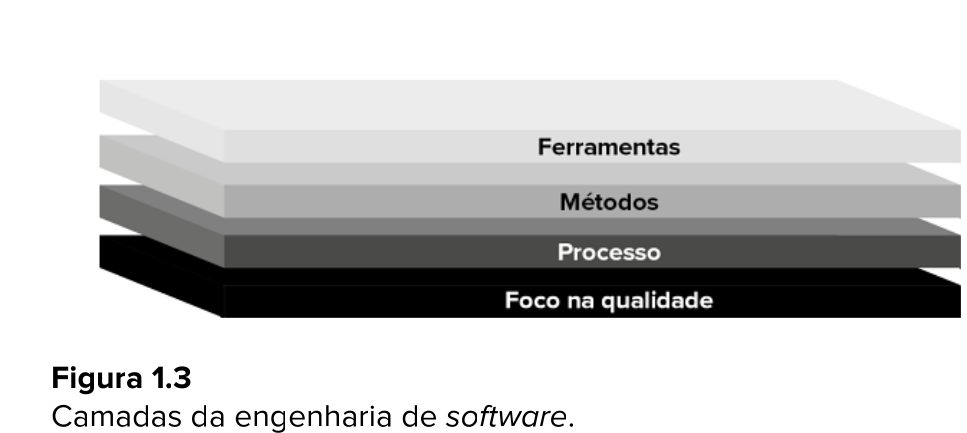
\includegraphics[width=0.72\textwidth]{image.png}
\end{center}

\vspace{0.2cm}
A ES é estruturada em quatro camadas; a \textbf{qualidade} é a base de toda a disciplina.
\end{frame}

%-------------------------------------------------------------
\begin{frame}
\frametitle{O Papel de Cada Camada}

\begin{center}
\begin{tikzpicture}[scale=0.82]
  \fill[yellow!25, rounded corners=3pt] (0,3.2) rectangle (10.2,4.0);
  \node[font=\scriptsize\bfseries, anchor=west] at (0.2,3.6) {Ferramentas --- automatizam (IDE, Git, CI/CD, modelagem)};

  \fill[orange!20, rounded corners=3pt] (0,2.2) rectangle (10.2,3.05);
  \node[font=\scriptsize\bfseries, anchor=west] at (0.2,2.625) {Métodos --- técnicas de análise, projeto, implementação e testes};

  \fill[cyan!18, rounded corners=3pt] (0,1.2) rectangle (10.2,2.05);
  \node[font=\scriptsize\bfseries, anchor=west] at (0.2,1.625) {Processo --- organiza e controla as etapas do desenvolvimento};

  \fill[structure.fg!25, rounded corners=3pt] (0,0.15) rectangle (10.2,1.05);
  \node[font=\scriptsize\bfseries, anchor=west] at (0.2,0.6) {Foco na Qualidade --- atender requisitos com confiabilidade};

  \draw[softarrow] (10.5,3.6) -- (10.5,0.6);
  \node[font=\tiny, rotate=90] at (10.85,2.1) {depende de};
\end{tikzpicture}
\end{center}

\begin{block}{Mensagem}
Qualidade nasce da integração processo + métodos + ferramentas --- não de uma camada isolada.
\end{block}
\end{frame}

%%%%%%%%%%%%%%%%%%%%%%%%%%%%%%%%%%%%%%%%%%%%%%%%%%%%%%%%%%%%%%
\section{1.3 O Processo de Software}

%-------------------------------------------------------------
\begin{frame}
\frametitle{1.3 O Processo de Software}

\begin{block}{Definição}
Conjunto organizado de \textbf{atividades}, \textbf{ações} e \textbf{tarefas}
para desenvolver um produto de software.
\end{block}

\begin{center}
\begin{tikzpicture}[scale=0.85]
  % Pirâmide de decomposição
  \fill[structure.fg!30] (2.5,2.8) -- (7.5,2.8) -- (6.5,3.6) -- (3.5,3.6) -- cycle;
  \node[font=\scriptsize\bfseries] at (5,3.2) {Processo};

  \fill[cyan!25] (1.5,1.6) -- (8.5,1.6) -- (7.5,2.6) -- (2.5,2.6) -- cycle;
  \node[font=\scriptsize\bfseries] at (5,2.1) {Atividades (objetivos amplos)};

  \fill[orange!22] (0.7,0.5) -- (9.3,0.5) -- (8.5,1.4) -- (1.5,1.4) -- cycle;
  \node[font=\scriptsize\bfseries] at (5,0.95) {Ações (conjuntos de tarefas)};

  \fill[yellow!25] (0, -0.6) -- (10,-0.6) -- (9.3,0.3) -- (0.7,0.3) -- cycle;
  \node[font=\scriptsize\bfseries] at (5,-0.15) {Tarefas (resultados específicos)};

  \node[font=\tiny] at (5,-1.05) {Do geral ao concreto: o processo se detalha até o trabalho diário};
\end{tikzpicture}
\end{center}
\end{frame}

%-------------------------------------------------------------
\begin{frame}
\frametitle{Atividade, Ação e Tarefa}

\begin{center}
\begin{tikzpicture}[scale=0.88]
  \node[draw, fill=structure.fg!20, rounded corners, text width=3.6cm, align=center, font=\scriptsize]
    (at) at (0,2.2) {\textbf{Atividade}\\Objetivo amplo\\ex.: Comunicação};
  \node[draw, fill=cyan!18, rounded corners, text width=3.6cm, align=center, font=\scriptsize]
    (ac) at (4.5,2.2) {\textbf{Ação}\\Conjunto de tarefas\\ex.: Levantar requisitos};
  \node[draw, fill=orange!18, rounded corners, text width=3.6cm, align=center, font=\scriptsize]
    (ta) at (9.0,2.2) {\textbf{Tarefa}\\Resultado específico\\ex.: Entrevistar usuários};

  \draw[softarrow] (at) -- (ac);
  \draw[softarrow] (ac) -- (ta);

  \node[draw=mRed, fill=mRed!8, rounded corners, text width=9cm, align=left, font=\tiny]
    at (4.5,0.5) {Analogia: \textbf{Atividade} = disciplina da faculdade;\quad
    \textbf{Ação} = unidade;\quad \textbf{Tarefa} = exercício da aula};
\end{tikzpicture}
\end{center}

\begin{tabular}{p{3cm}p{8cm}}
Atividade & Comunicação com o cliente \\
Ação & Levantamento de requisitos \\
Tarefa & Entrevistar usuários \\
\end{tabular}
\end{frame}

%-------------------------------------------------------------
\begin{frame}
\frametitle{As Cinco Atividades Metodológicas}

{\small Todo processo sério passa por estas cinco ``estações'' --- a ordem importa.}

\begin{center}
\begin{tikzpicture}[scale=0.82]
  \fill[yellow!30, rounded corners=3pt] (-0.15,0.8) rectangle (1.75,2.3);
  \node[font=\large\bfseries] at (0.8,1.9) {1};
  \node[font=\tiny\bfseries, align=center, text width=1.8cm] at (0.8,1.2) {Comunicação};

  \fill[orange!25, rounded corners=3pt] (2.05,0.8) rectangle (3.95,2.3);
  \node[font=\large\bfseries] at (3.0,1.9) {2};
  \node[font=\tiny\bfseries, align=center, text width=1.8cm] at (3.0,1.2) {Planejamento};

  \fill[cyan!25, rounded corners=3pt] (4.25,0.8) rectangle (6.15,2.3);
  \node[font=\large\bfseries] at (5.2,1.9) {3};
  \node[font=\tiny\bfseries, align=center, text width=1.8cm] at (5.2,1.2) {Modelagem};

  \fill[blue!20, rounded corners=3pt] (6.45,0.8) rectangle (8.35,2.3);
  \node[font=\large\bfseries] at (7.4,1.9) {4};
  \node[font=\tiny\bfseries, align=center, text width=1.8cm] at (7.4,1.2) {Construção};

  \fill[structure.fg!25, rounded corners=3pt] (8.65,0.8) rectangle (10.55,2.3);
  \node[font=\large\bfseries] at (9.6,1.9) {5};
  \node[font=\tiny\bfseries, align=center, text width=1.8cm] at (9.6,1.2) {Entrega};

  \draw[softarrow] (1.85,1.55) -- (2.05,1.55);
  \draw[softarrow] (4.05,1.55) -- (4.25,1.55);
  \draw[softarrow] (6.25,1.55) -- (6.45,1.55);
  \draw[softarrow] (8.45,1.55) -- (8.65,1.55);

  \node[font=\tiny] at (5.2,0.25)
    {Essas atividades aparecem em cascata, iterativo e ágil --- com ritmos diferentes};
\end{tikzpicture}
\end{center}
\end{frame}

%-------------------------------------------------------------
\begin{frame}
\frametitle{Comunicação e Planejamento}

\begin{columns}[T]
\column{0.48\textwidth}
\begin{block}{Comunicação}
Entender o problema, conversar com o cliente, levantar requisitos e definir objetivos.
\end{block}
\begin{block}{Planejamento}
Cronograma, custos, riscos e recursos.
\end{block}

\column{0.50\textwidth}
\centering
\begin{tikzpicture}[scale=0.85]
  \node[draw, fill=yellow!25, circle, minimum size=1.6cm, font=\scriptsize\bfseries] (cli) at (0,1.5) {Cliente};
  \node[draw, fill=structure.fg!22, circle, minimum size=1.6cm, font=\scriptsize\bfseries] (eq) at (4.2,1.5) {Equipe};

  \draw[softarrow] (cli) to[bend left=25] node[above,font=\tiny]{requisitos} (eq);
  \draw[softarrow] (eq) to[bend left=25] node[below,font=\tiny]{propostas} (cli);

  \node[draw=orange!80!black, fill=orange!12, rounded corners, text width=3.8cm, align=center, font=\tiny]
    at (2.1,-0.2) {Sem comunicação clara,\\o plano vira chute};
\end{tikzpicture}
\end{columns}
\end{frame}

%-------------------------------------------------------------
\begin{frame}
\frametitle{Modelagem, Construção e Entrega}

\begin{columns}[T]
\column{0.40\textwidth}
\begin{itemize}
\item \textbf{Modelagem:} UML, diagramas, arquitetura
\item \textbf{Construção:} programação e testes
\item \textbf{Entrega:} implantação e feedback
\end{itemize}

\column{0.58\textwidth}
\centering
\begin{tikzpicture}[scale=0.8]
  \node[draw, fill=orange!20, rounded corners, text width=2.4cm, align=center, font=\scriptsize\bfseries]
    (m) at (0,2.8) {Modelagem\\blueprint};
  \node[draw, fill=blue!18, rounded corners, text width=2.4cm, align=center, font=\scriptsize\bfseries]
    (c) at (0,1.4) {Construção\\código + testes};
  \node[draw, fill=structure.fg!22, rounded corners, text width=2.4cm, align=center, font=\scriptsize\bfseries]
    (e) at (0,0.0) {Entrega\\produto no ar};

  \draw[softarrow] (m)--(c);
  \draw[softarrow] (c)--(e);

  % mini UML hint
  \begin{scope}[shift={(3.2,1.5)}]
    \draw[thick, fill=white] (0,0) rectangle (2.8,2.2);
    \node[font=\tiny\bfseries] at (1.4,1.95) {UML (exemplo)};
    \draw (0.4,0.4) rectangle (1.3,1.5);
    \draw (1.6,0.7) rectangle (2.5,1.5);
    \draw[softarrow] (1.3,1.0) -- (1.6,1.0);
    \node[font=\tiny] at (1.4,-0.3) {modelo guia o código};
  \end{scope}
\end{tikzpicture}
\end{columns}

\begin{alertblock}{Resultado}
Cada iteração entrega um software mais completo e de maior qualidade.
\end{alertblock}
\end{frame}

%-------------------------------------------------------------
\begin{frame}
\frametitle{Desenvolvimento Iterativo}

{\small Em projetos modernos, as cinco atividades \textbf{se repetem} --- não acontecem uma vez só.}

\begin{center}
\begin{tikzpicture}[scale=0.78]
  \node[draw, fill=blue!12, rounded corners, minimum width=1.5cm, font=\tiny\bfseries] (n1) at (0.6,1.5) {Com.};
  \node[draw, fill=blue!12, rounded corners, minimum width=1.5cm, font=\tiny\bfseries] (n2) at (2.4,1.5) {Plan.};
  \node[draw, fill=blue!12, rounded corners, minimum width=1.5cm, font=\tiny\bfseries] (n3) at (4.2,1.5) {Mod.};
  \node[draw, fill=blue!12, rounded corners, minimum width=1.5cm, font=\tiny\bfseries] (n4) at (6.0,1.5) {Const.};
  \node[draw, fill=blue!12, rounded corners, minimum width=1.5cm, font=\tiny\bfseries] (n5) at (7.8,1.5) {Entr.};
  \draw[softarrow] (n1)--(n2);
  \draw[softarrow] (n2)--(n3);
  \draw[softarrow] (n3)--(n4);
  \draw[softarrow] (n4)--(n5);
  \draw[softarrowalert] (n5.south) to[bend left=45] node[below,font=\tiny\bfseries]{nova iteração} (n1.south);

  \node[draw, fill=structure.fg!15, rounded corners, font=\tiny] at (1.5,-0.3) {v0.1};
  \node[draw, fill=structure.fg!20, rounded corners, font=\tiny] at (4.2,-0.3) {v0.2};
  \node[draw, fill=structure.fg!30, rounded corners, font=\tiny] at (7.0,-0.3) {v1.0};
  \draw[softarrow] (1.9,-0.3)--(3.7,-0.3);
  \draw[softarrow] (4.7,-0.3)--(6.5,-0.3);
\end{tikzpicture}
\end{center}

\begin{block}{Benefícios}
Entregas frequentes $\cdot$ correções rápidas $\cdot$ feedback contínuo $\cdot$ menos risco
\end{block}
\end{frame}

%%%%%%%%%%%%%%%%%%%%%%%%%%%%%%%%%%%%%%%%%%%%%%%%%%%%%%%%%%%%%%
\section{Atividades de Apoio}

%-------------------------------------------------------------
\begin{frame}
\frametitle{1.3.2 Atividades de Apoio}

\begin{block}{Definição}
\textbf{Umbrella activities}: acompanham o projeto \textbf{do início ao fim}
(não são uma fase isolada).
\end{block}

\begin{center}
\begin{tikzpicture}[scale=0.8]
  % Linha do processo
  \draw[very thick, structure.fg] (0,1.5) -- (10,1.5);
  \node[draw, fill=white, rounded corners, font=\tiny] at (1,1.5) {Com.};
  \node[draw, fill=white, rounded corners, font=\tiny] at (3,1.5) {Plan.};
  \node[draw, fill=white, rounded corners, font=\tiny] at (5,1.5) {Mod.};
  \node[draw, fill=white, rounded corners, font=\tiny] at (7,1.5) {Const.};
  \node[draw, fill=white, rounded corners, font=\tiny] at (9,1.5) {Entr.};
  \node[font=\tiny\bfseries] at (5,2.0) {Atividades metodológicas (fluxo principal)};

  % Guarda-chuva
  \draw[thick, cyan!60!black, fill=cyan!12]
    (0.3,2.6) .. controls (5,4.0) and (5,4.0) .. (9.7,2.6) -- cycle;
  \node[font=\scriptsize\bfseries, cyan!60!black] at (5,3.2) {Atividades de Apoio};
  \node[font=\tiny] at (2.2,2.85) {controle};
  \node[font=\tiny] at (5.0,2.85) {qualidade};
  \node[font=\tiny] at (7.8,2.85) {mudanças/riscos};

  \node[font=\tiny, text width=10cm, align=center] at (5,0.6)
    {Enquanto o time desenvolve, o ``guarda-chuva'' protege prazo, qualidade e rastreabilidade};
\end{tikzpicture}
\end{center}
\end{frame}

%-------------------------------------------------------------
\begin{frame}
\frametitle{Controle e Acompanhamento do Projeto}

\begin{columns}[T]
\column{0.45\textwidth}
\begin{itemize}
\item Monitorar cronograma
\item Comparar plano $\times$ execução
\item Detectar atrasos cedo
\item Apoiar decisões
\end{itemize}
\begin{alertblock}{Resultado}
Corrigir desvios \textbf{antes} de virarem crise.
\end{alertblock}

\column{0.53\textwidth}
\centering
\begin{tikzpicture}[scale=0.85]
  \node[draw, fill=blue!15, rounded corners, minimum width=2.4cm, font=\scriptsize\bfseries] (p) at (0,2.4) {Plano};
  \node[draw, fill=orange!18, rounded corners, minimum width=2.4cm, font=\scriptsize\bfseries] (e) at (0,1.2) {Execução};
  \node[draw, fill=structure.fg!20, rounded corners, minimum width=2.4cm, font=\scriptsize\bfseries] (c) at (0,0.0) {Controle};

  \draw[softarrow] (p)--(e);
  \draw[softarrow] (e)--(c);
  \draw[dashed, softarrowalert] (c.east) to[bend left=50] node[right,font=\tiny]{ajuste} (p.east);

  % mini gráfico planejado vs real
  \begin{scope}[shift={(3.2,0.2)}]
    \draw[thick,->] (0,0)--(3.2,0);
    \draw[thick,->] (0,0)--(0,2.4);
    \draw[blue!70, thick] (0.2,0.3)--(1.2,1.0)--(2.2,1.6)--(3.0,2.1);
    \draw[mRed, thick, dashed] (0.2,0.3)--(1.2,0.7)--(2.2,1.1)--(3.0,1.3);
    \node[font=\tiny,blue!70] at (2.0,2.3) {plano};
    \node[font=\tiny,mRed] at (2.6,0.9) {real};
  \end{scope}
\end{tikzpicture}
\end{columns}
\end{frame}

%-------------------------------------------------------------
\begin{frame}
\frametitle{Administração de Riscos}

\begin{block}{Objetivo}
Identificar, analisar e minimizar ameaças ao produto/projeto.
\end{block}

\begin{center}
\begin{tikzpicture}[scale=0.85]
  \node[draw, fill=yellow!30, circle, minimum size=1.7cm, font=\scriptsize\bfseries, align=center]
    (id) at (1,1.5) {1\\Identificar};
  \node[draw, fill=orange!30, circle, minimum size=1.7cm, font=\scriptsize\bfseries, align=center]
    (an) at (4.5,1.5) {2\\Analisar};
  \node[draw, fill=structure.fg!30, circle, minimum size=1.7cm, font=\scriptsize\bfseries, align=center]
    (mi) at (8,1.5) {3\\Mitigar};

  \draw[softarrow] (id)--(an);
  \draw[softarrow] (an)--(mi);
  \draw[dashed, softarrowalert] (mi.south) to[bend left=40] node[below,font=\tiny]{monitorar de novo} (id.south);
\end{tikzpicture}
\end{center}

{\scriptsize Exemplos: perda de pessoas, mudança de requisitos, atraso, falha tecnológica.}
\end{frame}

%-------------------------------------------------------------
\begin{frame}
\frametitle{Garantia da Qualidade e Revisões Técnicas}

\begin{columns}[T]
\column{0.48\textwidth}
\textbf{Garantia da Qualidade}\\{\scriptsize normas, padrões, auditorias, melhoria contínua}
\vspace{0.3cm}

\textbf{Revisões Técnicas}\\{\scriptsize requisitos, projeto, código, inspeções}

\column{0.50\textwidth}
\centering
\begin{tikzpicture}[scale=0.85]
  \node[draw, fill=structure.fg!15, rounded corners, text width=2.2cm, align=center, font=\scriptsize]
    (a) at (0,2.0) {Artefato\\(código, doc)};
  \node[draw, fill=yellow!25, rounded corners, text width=2.2cm, align=center, font=\scriptsize\bfseries]
    (r) at (0,0.7) {Revisão\\técnica};
  \node[draw, fill=cyan!20, rounded corners, text width=2.2cm, align=center, font=\scriptsize]
    (p) at (0,-0.6) {Produto\\mais confiável};

  \draw[softarrow] (a)--(r);
  \draw[softarrow] (r)--(p);
  \draw[dashed, softarrowalert] (r.east) to[bend left=40] node[right,font=\tiny]{achou defeito} (a.east);
\end{tikzpicture}
\end{columns}
\end{frame}

%-------------------------------------------------------------
\begin{frame}
\frametitle{Medição e Gerência da Configuração}

\begin{columns}[T]
\column{0.42\textwidth}
\textbf{Medição}\\{\scriptsize produtividade, defeitos, esforço, custo, qualidade}
\vspace{0.25cm}

\textbf{Configuração}\\{\scriptsize versões, histórico, mudanças, rastreabilidade}

\column{0.56\textwidth}
\centering
\begin{tikzpicture}[scale=0.85]
  % Linha do tempo de versões (Git-like)
  \draw[very thick, gray] (0,1.2)--(6.5,1.2);
  \foreach \x/\v/\c in {0.5/v1.0/blue!20,2.5/v1.1/cyan!20,4.5/v2.0/structure.fg!25,6.2/hotfix/orange!25}{
    \fill[\c] (\x,1.2) circle (0.18);
    \node[font=\tiny\bfseries] at (\x,1.7) {\v};
  }
  \draw[softarrow] (0.7,1.2)--(2.3,1.2);
  \draw[softarrow] (2.7,1.2)--(4.3,1.2);
  \draw[softarrowalert] (4.7,1.2)--(6.0,1.2);

  \node[font=\tiny, text width=5.5cm, align=center] at (3.2,0.4)
    {Medir para decidir; versionar para não perder o controle};
\end{tikzpicture}
\end{columns}
\end{frame}

%-------------------------------------------------------------
\begin{frame}
\frametitle{Reutilização e Produção de Artefatos}

\begin{columns}[T]
\column{0.42\textwidth}
\textbf{Reutilização}\\{\scriptsize bibliotecas, componentes, APIs, frameworks}
\vspace{0.2cm}

\textbf{Artefatos}\\{\scriptsize docs, UML, testes, manuais}

\column{0.56\textwidth}
\centering
\begin{tikzpicture}[scale=0.8]
  \node[draw=structure.fg, fill=structure.fg!25, rounded corners, minimum width=2.8cm, font=\scriptsize\bfseries]
    (comp) at (2.5,2.6) {Componente};
  \node[draw, fill=blue!12, rounded corners, font=\tiny] (a) at (0,0.8) {Projeto A};
  \node[draw, fill=blue!12, rounded corners, font=\tiny] (b) at (2.5,0.8) {Projeto B};
  \node[draw, fill=blue!12, rounded corners, font=\tiny] (c) at (5.0,0.8) {Projeto C};
  \draw[softarrow] (comp)--(a);
  \draw[softarrow] (comp)--(b);
  \draw[softarrow] (comp)--(c);
  \node[font=\tiny] at (2.5,0.1) {escrever uma vez, usar várias};
\end{tikzpicture}
\end{columns}

\begin{block}{Mensagem}
Apoio ao longo do ciclo de vida $\Rightarrow$ mais qualidade, menos risco, manutenção mais fácil.
\end{block}
\end{frame}

%%%%%%%%%%%%%%%%%%%%%%%%%%%%%%%%%%%%%%%%%%%%%%%%%%%%%%%%%%%%%%
\section{1.3.3 Adaptação do Processo}

%-------------------------------------------------------------
\begin{frame}
\frametitle{1.3.3 Adaptação do Processo}

\begin{block}{Ideia central}
Não copie o processo ``de livro'' no piloto automático ---
\textbf{customize} ao projeto, à equipe e à organização.
\end{block}

\begin{center}
\begin{tikzpicture}[scale=0.88]
  \node[draw, fill=blue!15, rounded corners, text width=2.8cm, align=center, font=\scriptsize\bfseries]
    (g) at (0,1.2) {Processo\\genérico};
  \node[draw, fill=orange!20, rounded corners, text width=2.6cm, align=center, font=\tiny]
    (f) at (4.0,2.4) {tamanho};
  \node[draw, fill=orange!20, rounded corners, text width=2.6cm, align=center, font=\tiny]
    (f2) at (4.0,1.2) {prazo / risco};
  \node[draw, fill=orange!20, rounded corners, text width=2.6cm, align=center, font=\tiny]
    (f3) at (4.0,0.0) {equipe / cliente};
  \node[draw, fill=structure.fg!25, rounded corners, text width=2.8cm, align=center, font=\scriptsize\bfseries]
    (a) at (8.0,1.2) {Processo\\adaptado};

  \draw[softarrow] (g)--(4.0,1.2);
  \draw[softarrow] (f)--(a);
  \draw[softarrow] (f2)--(a);
  \draw[softarrow] (f3)--(a);
\end{tikzpicture}
\end{center}
\end{frame}

%-------------------------------------------------------------
\begin{frame}
\frametitle{Por que Adaptar o Processo?}

{\small Um único processo \textbf{não} serve igualmente a todos os projetos.}

\begin{center}
\begin{tikzpicture}[scale=0.85]
  \node[draw=structure.fg, fill=structure.fg!20, circle, minimum size=1.9cm, font=\scriptsize\bfseries]
    (p) at (4.5,1.8) {Projeto};

  \node[draw, fill=cyan!15, rounded corners, font=\tiny] (t) at (0.5,3.2) {Tamanho};
  \node[draw, fill=cyan!15, rounded corners, font=\tiny] (c) at (4.5,3.4) {Complexidade};
  \node[draw, fill=cyan!15, rounded corners, font=\tiny] (z) at (8.5,3.2) {Prazo};
  \node[draw, fill=cyan!15, rounded corners, font=\tiny] (e) at (1.5,0.2) {Equipe};
  \node[draw, fill=cyan!15, rounded corners, font=\tiny] (cl) at (7.5,0.2) {Cliente};

  \foreach \n in {t,c,z,e,cl}
    \draw[softarrow] (p)--(\n);
\end{tikzpicture}
\end{center}
\end{frame}

%-------------------------------------------------------------
\begin{frame}
\frametitle{Fatores que Influenciam a Adaptação}

\begin{center}
\begin{tikzpicture}[scale=0.82,
  h/.style={font=\scriptsize\bfseries},
  c/.style={font=\tiny, text width=3.6cm, align=left},
  f/.style={font=\tiny\bfseries, text width=2.6cm, align=center}
]
\node[h] at (1.5,3.3) {Fator};
\node[h] at (6.0,3.3) {Impacto no processo};
\draw[structure.fg!40] (-0.2,3.0)--(9.5,3.0);

\node[f] at (1.5,2.4) {Tamanho};
\node[c] at (6.0,2.4) {Mais documentação e controle};

\node[f] at (1.5,1.7) {Complexidade};
\node[c] at (6.0,1.7) {Mais análise e projeto};

\node[f] at (1.5,1.0) {Equipe / Cliente};
\node[c] at (6.0,1.0) {Comunicação e participação};

\node[f] at (1.5,0.3) {Prazo / Organização};
\node[c] at (6.0,0.3) {Nº de iterações; normas da empresa};
\end{tikzpicture}
\end{center}

\vspace{0.2cm}
{\small Quanto maior a complexidade, maior tende a ser o \textbf{rigor} do processo.}
\end{frame}

%-------------------------------------------------------------
\begin{frame}
\frametitle{Projeto Pequeno × Projeto Grande}

\begin{center}
\begin{tikzpicture}[scale=0.85]
  \fill[structure.fg!12, rounded corners=4pt] (0,0) rectangle (4.6,3.6);
  \fill[orange!12, rounded corners=4pt] (5.4,0) rectangle (10.0,3.6);

  \node[font=\small\bfseries] at (2.3,3.2) {Projeto pequeno};
  \node[font=\small\bfseries] at (7.7,3.2) {Projeto grande};

  \node[font=\scriptsize, align=left, text width=4.0cm] at (2.3,1.6) {
    $\bullet$ equipe reduzida\\
    $\bullet$ pouca documentação\\
    $\bullet$ processo ágil\\
    $\bullet$ menos burocracia
  };
  \node[font=\scriptsize, align=left, text width=4.0cm] at (7.7,1.6) {
    $\bullet$ várias equipes\\
    $\bullet$ documentação extensa\\
    $\bullet$ planejamento detalhado\\
    $\bullet$ gestão de riscos forte
  };

  \draw[<->, thick, mRed] (4.7,1.8)--(5.3,1.8);
  \node[font=\tiny\bfseries, mRed] at (5.0,2.2) {escala};
\end{tikzpicture}
\end{center}
\end{frame}

%-------------------------------------------------------------
\begin{frame}
\frametitle{Níveis de Adaptação}

{\small Você pode ``afinar'' o processo em quatro eixos:}

\begin{center}
\begin{tikzpicture}[scale=0.85]
  \node[draw=structure.fg, fill=structure.fg!22, circle, minimum size=2.0cm, font=\scriptsize\bfseries]
    (p) at (4.5,1.8) {Processo};

  \node[draw, fill=orange!18, rounded corners, text width=2.4cm, align=center, font=\tiny]
    (f) at (0.5,3.2) {\textbf{Fluxo}\\quais atividades e quando};
  \node[draw, fill=orange!18, rounded corners, text width=2.4cm, align=center, font=\tiny]
    (a) at (8.5,3.2) {\textbf{Artefatos}\\quanto documentar};
  \node[draw, fill=orange!18, rounded corners, text width=2.4cm, align=center, font=\tiny]
    (q) at (0.5,0.3) {\textbf{Qualidade}\\nível de rigor};
  \node[draw, fill=orange!18, rounded corners, text width=2.4cm, align=center, font=\tiny]
    (e) at (8.5,0.3) {\textbf{Equipe}\\papéis e comunicação};

  \foreach \n in {f,a,q,e}
    \draw[softarrow] (p)--(\n);
\end{tikzpicture}
\end{center}
\end{frame}

%-------------------------------------------------------------
\begin{frame}
\frametitle{Exemplo de Adaptação}

\begin{block}{Caso ágil}
Ciclos curtos + feedback do cliente a cada entrega.
\end{block}

\begin{center}
\begin{tikzpicture}[scale=0.78]
  \node[draw, fill=structure.fg!18, rounded corners, minimum width=1.5cm, font=\tiny\bfseries] (a1) at (0.8,1.6) {Com.};
  \node[draw, fill=structure.fg!18, rounded corners, minimum width=1.5cm, font=\tiny\bfseries] (a2) at (2.6,1.6) {Plan.};
  \node[draw, fill=structure.fg!18, rounded corners, minimum width=1.5cm, font=\tiny\bfseries] (a3) at (4.4,1.6) {Mod.};
  \node[draw, fill=structure.fg!18, rounded corners, minimum width=1.5cm, font=\tiny\bfseries] (a4) at (6.2,1.6) {Const.};
  \node[draw, fill=structure.fg!18, rounded corners, minimum width=1.5cm, font=\tiny\bfseries] (a5) at (8.0,1.6) {Entr.};
  \draw[softarrow] (a1)--(a2);
  \draw[softarrow] (a2)--(a3);
  \draw[softarrow] (a3)--(a4);
  \draw[softarrow] (a4)--(a5);
  \draw[softarrowalert] (a5.south) to[bend left=40] node[below,font=\tiny\bfseries]{feedback} (a1.south);
  \node[font=\tiny] at (4.4,0.2) {Cada volta = nova versão utilizável};
\end{tikzpicture}
\end{center}
\end{frame}

%-------------------------------------------------------------
\begin{frame}
\frametitle{Resumo da Adaptação do Processo}

\begin{center}
\begin{tikzpicture}[scale=0.85]
  \node[draw, fill=yellow!20, rounded corners, text width=8.5cm, align=left, font=\scriptsize]
    at (0,2.2) {
    $\bullet$ Não existe processo único para todos\\
    $\bullet$ Flexibilidade reduz desperdício\\
    $\bullet$ Rigor depende do contexto\\
    $\bullet$ Meta constante: software de qualidade
  };
  \node[draw=structure.fg, fill=structure.fg!18, rounded corners, text width=8.5cm, align=center, font=\small\bfseries]
    at (0,0.4) {Processos eficazes se adaptam ao problema,\\não o contrário.};
\end{tikzpicture}
\end{center}
\end{frame}

%%%%%%%%%%%%%%%%%%%%%%%%%%%%%%%%%%%%%%%%%%%%%%%%%%%%%%%%%%%%%%
\section{1.4 A Prática da Engenharia de Software}

%-------------------------------------------------------------
\begin{frame}
\frametitle{1.4 A Prática da Engenharia de Software}

\begin{block}{O que é?}
Aplicar \textbf{processos + métodos + ferramentas} para produzir software
de forma organizada, previsível e com qualidade.
\end{block}

\begin{center}
\begin{tikzpicture}[scale=0.8]
  \node[draw, fill=blue!15, rounded corners, font=\tiny\bfseries] (p) at (0,1.5) {Processo};
  \node[draw, fill=orange!18, rounded corners, font=\tiny\bfseries] (m) at (3.0,1.5) {Métodos};
  \node[draw, fill=cyan!18, rounded corners, font=\tiny\bfseries] (f) at (6.0,1.5) {Ferramentas};
  \node[draw=structure.fg, fill=structure.fg!25, rounded corners, font=\scriptsize\bfseries] (pr) at (9.0,1.5) {Prática};

  \draw[softarrow] (p)--(pr);
  \draw[softarrow] (m)--(pr);
  \draw[softarrow] (f)--(pr);

  \node[font=\tiny] at (4.5,0.5) {+ comunicação, planejamento, modelagem, construção, entrega e apoio};
\end{tikzpicture}
\end{center}
\end{frame}

%-------------------------------------------------------------
\begin{frame}
\frametitle{A Engenharia de Software na Prática}

\begin{center}
\begin{tikzpicture}[scale=0.78]
  \node[draw, fill=yellow!30, rounded corners, minimum width=1.9cm, text width=1.7cm, align=center, font=\tiny\bfseries]
    (p1) at (0.8,1.6) {Comunicação};
  \node[draw, fill=orange!25, rounded corners, minimum width=1.9cm, text width=1.7cm, align=center, font=\tiny\bfseries]
    (p2) at (3.0,1.6) {Planejamento};
  \node[draw, fill=cyan!25, rounded corners, minimum width=1.9cm, text width=1.7cm, align=center, font=\tiny\bfseries]
    (p3) at (5.2,1.6) {Modelagem};
  \node[draw, fill=blue!20, rounded corners, minimum width=1.9cm, text width=1.7cm, align=center, font=\tiny\bfseries]
    (p4) at (7.4,1.6) {Construção};
  \node[draw, fill=structure.fg!25, rounded corners, minimum width=1.9cm, text width=1.7cm, align=center, font=\tiny\bfseries]
    (p5) at (9.6,1.6) {Entrega};
  \draw[softarrow] (p1)--(p2);
  \draw[softarrow] (p2)--(p3);
  \draw[softarrow] (p3)--(p4);
  \draw[softarrow] (p4)--(p5);
  \draw[softarrowalert] (p5.south) to[bend left=35] node[below,font=\tiny]{feedback / aprendizado} (p1.south);
\end{tikzpicture}
\end{center}

\vspace{0.3cm}
Cada entrega gera aprendizado para a próxima iteração.
\end{frame}

%%%%%%%%%%%%%%%%%%%%%%%%%%%%%%%%%%%%%%%%%%%%%%%%%%%%%%%%%%%%%%
\section{1.4.1 A Essência da Prática}

%-------------------------------------------------------------
\begin{frame}
\frametitle{1.4.1 A Essência da Prática}

George Polya: estratégia geral de resolução de problemas --- aplicável ao software.

\begin{center}
\begin{tikzpicture}[scale=0.85]
  \fill[yellow!30, rounded corners=4pt] (0.1,0.6) rectangle (2.3,2.4);
  \node[font=\Large\bfseries] at (1.2,1.9) {1};
  \node[font=\scriptsize\bfseries] at (1.2,1.1) {Compreender};

  \fill[orange!25, rounded corners=4pt] (2.9,0.6) rectangle (5.1,2.4);
  \node[font=\Large\bfseries] at (4.0,1.9) {2};
  \node[font=\scriptsize\bfseries] at (4.0,1.1) {Planejar};

  \fill[cyan!25, rounded corners=4pt] (5.7,0.6) rectangle (7.9,2.4);
  \node[font=\Large\bfseries] at (6.8,1.9) {3};
  \node[font=\scriptsize\bfseries] at (6.8,1.1) {Executar};

  \fill[structure.fg!25, rounded corners=4pt] (8.5,0.6) rectangle (10.7,2.4);
  \node[font=\Large\bfseries] at (9.6,1.9) {4};
  \node[font=\scriptsize\bfseries] at (9.6,1.1) {Examinar};

  \draw[softarrow] (2.4,1.5)--(2.85,1.5);
  \draw[softarrow] (5.2,1.5)--(5.65,1.5);
  \draw[softarrow] (8.0,1.5)--(8.45,1.5);
\end{tikzpicture}
\end{center}
\end{frame}

%-------------------------------------------------------------
\begin{frame}
\frametitle{1º Passo: Compreender o Problema}

\begin{alertblock}{Objetivo}
Entender certo \textbf{antes} de codar --- evita retrabalho.
\end{alertblock}

\begin{center}
\begin{tikzpicture}[scale=0.85]
  \node[draw=mRed, fill=mRed!10, rounded corners, text width=2.6cm, align=center, font=\scriptsize\bfseries]
    (prob) at (0,1.5) {Problema\\mal definido};
  \node[draw, fill=yellow!25, rounded corners, text width=3.2cm, align=left, font=\tiny]
    (q) at (4.5,1.5) {
    Quem são os envolvidos?\\
    Quais objetivos?\\
    Que dados faltam?\\
    Dá para dividir?\\
    Dá para diagramar?
  };
  \node[draw=structure.fg, fill=structure.fg!18, rounded corners, text width=2.6cm, align=center, font=\scriptsize\bfseries]
    (ok) at (9.0,1.5) {Problema\\compreendido};

  \draw[softarrow] (prob)--(q);
  \draw[softarrow] (q)--(ok);
\end{tikzpicture}
\end{center}
\end{frame}

%-------------------------------------------------------------
\begin{frame}
\frametitle{2º Passo: Planejar a Solução}

\begin{center}
\begin{tikzpicture}[scale=0.85]
  \node[draw, fill=mRed!12, rounded corners, font=\scriptsize\bfseries] (p) at (0,1.5) {Problema};
  \node[draw, fill=orange!20, rounded corners, text width=2.4cm, align=center, font=\scriptsize\bfseries]
    (m) at (4.0,1.5) {Projeto /\\estratégia};
  \node[draw, fill=structure.fg!22, rounded corners, font=\scriptsize\bfseries] (s) at (8.0,1.5) {Solução};

  \draw[softarrow] (p)--node[above,font=\tiny]{buscar padrões} (m);
  \draw[softarrow] (m)--node[above,font=\tiny]{definir caminho} (s);

  \node[font=\tiny, text width=9cm, align=center] at (4.0,0.3)
    {Reuso, arquitetura adequada, divisão em subproblemas};
\end{tikzpicture}
\end{center}
\end{frame}

%-------------------------------------------------------------
\begin{frame}
\frametitle{3º Passo: Executar o Plano}

{\small Aqui a solução vira software de verdade.}

\begin{center}
\begin{tikzpicture}[scale=0.85]
  \node[draw, fill=orange!20, rounded corners, font=\scriptsize\bfseries] (proj) at (0,2.0) {Projeto};
  \node[draw, fill=blue!18, rounded corners, font=\scriptsize\bfseries] (cod) at (4.0,2.0) {Código};
  \node[draw, fill=cyan!18, rounded corners, font=\scriptsize\bfseries] (int) at (8.0,2.0) {Integração};

  \draw[softarrow] (proj)--(cod);
  \draw[softarrow] (cod)--(int);

  \node[draw, fill=yellow!20, rounded corners, font=\tiny] (t) at (2.0,0.4) {testes de unidade};
  \node[draw, fill=yellow!20, rounded corners, font=\tiny] (r) at (5.0,0.4) {revisão de código};
  \node[draw, fill=yellow!20, rounded corners, font=\tiny] (f) at (8.0,0.4) {correção de defeitos};

  \draw[softarrow] (cod)--(t);
  \draw[softarrow] (cod)--(r);
  \draw[softarrow] (int)--(f);
\end{tikzpicture}
\end{center}
\end{frame}

%-------------------------------------------------------------
\begin{frame}
\frametitle{4º Passo: Examinar os Resultados}

\begin{columns}[T]
\column{0.45\textwidth}
\begin{itemize}
\item Testes
\item Validação
\item Verificação
\item Correção de erros
\end{itemize}
{\small O software atende aos requisitos dos usuários?}

\column{0.53\textwidth}
\centering
\begin{tikzpicture}[scale=0.85]
  \node[draw, fill=structure.fg!20, rounded corners, font=\scriptsize\bfseries] (s) at (1.5,2.4) {Software};
  \node[draw, fill=cyan!20, rounded corners, font=\scriptsize\bfseries] (t) at (1.5,1.2) {Testes};
  \node[draw, fill=yellow!25, rounded corners, font=\scriptsize\bfseries] (q) at (1.5,0.0) {Qualidade};

  \draw[softarrow] (s)--(t);
  \draw[softarrow] (t)--(q);

  \node[draw=mRed, fill=mRed!10, rounded corners, text width=2.2cm, align=center, font=\tiny]
    (fail) at (4.5,1.2) {falhou?\\volte e corrija};
  \draw[dashed, softarrowalert] (t)--(fail);
  \draw[dashed, softarrowalert] (fail.north) to[bend right=20] (s.east);
\end{tikzpicture}
\end{columns}
\end{frame}

%-------------------------------------------------------------
\begin{frame}
\frametitle{A Essência da Engenharia de Software}

\begin{center}
\begin{tikzpicture}[scale=0.85]
  \node[draw, fill=yellow!30, rounded corners, minimum width=2.4cm, font=\scriptsize\bfseries] (c) at (0,2.5) {Compreender};
  \node[draw, fill=orange!25, rounded corners, minimum width=2.4cm, font=\scriptsize\bfseries] (p) at (0,1.5) {Planejar};
  \node[draw, fill=cyan!25, rounded corners, minimum width=2.4cm, font=\scriptsize\bfseries] (e) at (0,0.5) {Executar};
  \node[draw, fill=structure.fg!25, rounded corners, minimum width=2.4cm, font=\scriptsize\bfseries] (x) at (0,-0.5) {Examinar};

  \draw[softarrow] (c)--(p);
  \draw[softarrow] (p)--(e);
  \draw[softarrow] (e)--(x);
  \draw[softarrowalert] (x.east) to[bend left=55] node[right,font=\tiny\bfseries]{melhoria contínua} (c.east);

  \node[draw, fill=blue!10, rounded corners, text width=4.5cm, align=left, font=\tiny]
    at (5.5,1.0) {
    Cada ciclo:\\
    $\bullet$ gera conhecimento\\
    $\bullet$ melhora qualidade\\
    $\bullet$ reduz riscos
  };
\end{tikzpicture}
\end{center}

\begin{block}{Mensagem}
A ES é resolução de problemas \textbf{iterativa}, não uma receita linear única.
\end{block}
\end{frame}

%-------------------------------------------------------------
\begin{frame}
\frametitle{Resumo do Capítulo}

\begin{center}
\begin{tikzpicture}[scale=0.78]
  \node[draw, fill=structure.fg!20, rounded corners, text width=2.3cm, align=center, font=\tiny\bfseries]
    (es) at (0,1.5) {Engenharia\\de Software};
  \node[draw, fill=cyan!18, rounded corners, text width=2.3cm, align=center, font=\tiny\bfseries]
    (pr) at (3.2,1.5) {Processo\\orienta};
  \node[draw, fill=orange!18, rounded corners, text width=2.3cm, align=center, font=\tiny\bfseries]
    (ap) at (6.4,1.5) {Apoio\\protege};
  \node[draw, fill=yellow!25, rounded corners, text width=2.3cm, align=center, font=\tiny\bfseries]
    (ad) at (9.6,1.5) {Adaptação\\contextualiza};

  \draw[softarrow] (es)--(pr);
  \draw[softarrow] (pr)--(ap);
  \draw[softarrow] (ap)--(ad);

  \node[draw=structure.fg, fill=structure.fg!12, rounded corners, text width=10cm, align=center, font=\scriptsize]
    at (4.8,0.1) {Prática: compreender $\rightarrow$ planejar $\rightarrow$ executar $\rightarrow$ examinar (e repetir)};
\end{tikzpicture}
\end{center}

\begin{itemize}
\item ES é disciplina organizada; o processo guia o desenvolvimento.
\item Atividades de apoio sustentam qualidade e controle.
\item O processo se adapta ao projeto.
\item A prática é ciclo contínuo de resolução de problemas.
\end{itemize}
\end{frame}

\end{document}
